% -*- coding: utf-8 -*-
%\documentclass[output=paper]{LSP/langsci} 
\documentclass[output=paper
,newtxmath
,modfonts
,nonflat]{langsci/langscibook} 
% \bibliography{localbibliography} 
% \usepackage{pifont}
\usepackage{savesym}

\savesymbol{downingtriple}
\savesymbol{downingdouble}
\savesymbol{downingquad}
\savesymbol{downingquint}
\savesymbol{suph}
\savesymbol{supj}
\savesymbol{supw}
\savesymbol{sups}
\savesymbol{ts}
\savesymbol{tS}
\savesymbol{devi}
\savesymbol{devu}
\savesymbol{devy}
\savesymbol{deva}
\savesymbol{N}
\savesymbol{Z}
\savesymbol{circled}
\savesymbol{sem}
\savesymbol{row}
\savesymbol{tipa}
\savesymbol{tableauxcounter}
\savesymbol{tabhead}
\savesymbol{inp}
\savesymbol{inpno}
\savesymbol{g}
\savesymbol{hanl}
\savesymbol{hanr}
\savesymbol{kuku}
\savesymbol{ip}
\savesymbol{lipm}
\savesymbol{ripm}
\savesymbol{lipn}
\savesymbol{ripn} 
% \usepackage{amsmath} 
% \usepackage{multicol}
\usepackage{qtree} 
\usepackage{tikz-qtree,tikz-qtree-compat}
% \usepackage{tikz}
\usepackage{upgreek}


%%%%%%%%%%%%%%%%%%%%%%%%%%%%%%%%%%%%%%%%%%%%%%%%%%%%
%%%                                              %%%
%%%           Examples                           %%%
%%%                                              %%%
%%%%%%%%%%%%%%%%%%%%%%%%%%%%%%%%%%%%%%%%%%%%%%%%%%%%
% remove the percentage signs in the following lines
% if your book makes use of linguistic examples
\usepackage{tipa}  
\usepackage{pstricks,pst-xkey,pst-asr}

%for sande et al
\usepackage{pst-jtree}
\usepackage{pst-node}
%\usepackage{savesym}


% \usepackage{subcaption}
\usepackage{multirow}  
\usepackage{./langsci/styles/langsci-optional} 
\usepackage{./langsci/styles/langsci-lgr} 
\usepackage{./langsci/styles/langsci-glyphs} 
\usepackage[normalem]{ulem}
%% if you want the source line of examples to be in italics, uncomment the following line
% \def\exfont{\it}
\usetikzlibrary{arrows.meta,topaths,trees}
\usepackage[linguistics]{forest}
\forestset{
	fairly nice empty nodes/.style={
		delay={where content={}{shape=coordinate,for parent={
					for children={anchor=north}}}{}}
}}
\usepackage{soul}
\usepackage{arydshln}
% \usepackage{subfloat}
\usepackage{langsci/styles/langsci-gb4e} 
   
% \usepackage{linguex}
\usepackage{vowel}

\usepackage{pifont}% http://ctan.org/pkg/pifont
\newcommand{\cmark}{\ding{51}}%
\newcommand{\xmark}{\ding{55}}%
 
 
 %Lamont
 \makeatletter
\g@addto@macro\@floatboxreset\centering
\makeatother

\usepackage{newfloat} 
\DeclareFloatingEnvironment[fileext=tbx,name=Tableau]{tableau}
% %% hyphenation points for line breaks
%% Normally, automatic hyphenation in LaTeX is very good
%% If a word is mis-hyphenated, add it to this file
%%
%% add information to TeX file before \begin{document} with:
%% %% hyphenation points for line breaks
%% Normally, automatic hyphenation in LaTeX is very good
%% If a word is mis-hyphenated, add it to this file
%%
%% add information to TeX file before \begin{document} with:
%% %% hyphenation points for line breaks
%% Normally, automatic hyphenation in LaTeX is very good
%% If a word is mis-hyphenated, add it to this file
%%
%% add information to TeX file before \begin{document} with:
%% \include{localhyphenation}
\hyphenation{
affri-ca-te
affri-ca-tes
com-ple-ments
par-a-digm
Sha-ron
Kings-ton
phe-nom-e-non
Daul-ton
Abu-ba-ka-ri
Ngo-nya-ni
Clem-ents 
King-ston
Tru-cken-brodt
Tab-leau
cophono-logies
mark-edness
Ti-gri-nya
a-mong
Car-stens
Lu-bu-ku-su
}
\hyphenation{
affri-ca-te
affri-ca-tes
com-ple-ments
par-a-digm
Sha-ron
Kings-ton
phe-nom-e-non
Daul-ton
Abu-ba-ka-ri
Ngo-nya-ni
Clem-ents 
King-ston
Tru-cken-brodt
Tab-leau
cophono-logies
mark-edness
Ti-gri-nya
a-mong
Car-stens
Lu-bu-ku-su
}
\hyphenation{
affri-ca-te
affri-ca-tes
com-ple-ments
par-a-digm
Sha-ron
Kings-ton
phe-nom-e-non
Daul-ton
Abu-ba-ka-ri
Ngo-nya-ni
Clem-ents 
King-ston
Tru-cken-brodt
Tab-leau
cophono-logies
mark-edness
Ti-gri-nya
a-mong
Car-stens
Lu-bu-ku-su
}
% %add all your local new commands to this file
\newcommand{\downingquad}[4]{\parbox{2.5cm}{#1}\parbox{3.5cm}{#2}\parbox{2.5cm}{#3}\parbox{3.5cm}{#4}}
\newcommand{\downingtriple}[3]{\parbox{4.5cm}{#1}\parbox{3cm}{#2}\parbox{3cm}{#3}}
\newcommand{\downingdouble}[2]{\parbox{4.5cm}{#1}\parbox{6cm}{#2}}
\newcommand{\downingquint}[5]{\parbox{1.75cm}{#1}\parbox{2.25cm}{#2}\parbox{2cm}{#3}\parbox{3cm}{#4}\parbox{2cm}{#5}}
\newcolumntype{Y}{>{\centering\arraybackslash}X}
\newcolumntype{T}{>{\centering\arraybackslash}m{2cm}}

%commands for Kusmer paper below
\newcommand{\ip}{$\upiota$}
\newcommand{\lipm}{(\_{\ip-Max}}
\newcommand{\ripm}{)\_{\ip-Max}}
\newcommand{\lipn}{(\_{\ip}}
\newcommand{\ripn}{)\_{\ip}}
\renewcommand{\_}[1]{\textsubscript{#1}}


%commands for Pillion paper below
\newcommand{\suph}{\textipa{\super h}}
\newcommand{\supj}{\textipa{\super j}}
\newcommand{\supw}{\textipa{\super w}}
\newcommand{\ts}{\textipa{\t{ts}}}
\newcommand{\tS}{\textipa{\t{tS}}}
\newcommand{\devi}{\textipa{\r*i}}
\newcommand{\devu}{\textipa{\r*u}}
\newcommand{\devy}{\textipa{\r*y}}
\newcommand{\deva}{\textipa{\r*a}}
\renewcommand{\N}{\textipa{N}}
\newcommand{\Z}{\textipa{Z}}
% 

%commands for Diercks paper below
\newcommand{\circled}[1]{\begin{tikzpicture}[baseline=(word.base)]
\node[draw, rounded corners, text height=8pt, text depth=2pt, inner sep=2pt, outer sep=0pt, use as bounding box] (word) {#1};
\end{tikzpicture}
}

%commands for Pesetsky paper below
% \newcommand{\sem}[2][]{\mbox{$[\![ $\textbf{#2}$ ]\!]^{#1}$}}
\newcommand{\sem}[2][]{\mbox{$[[ $\textbf{#2}$ ]]^{#1}$}}

% \newcommand{\ripn}{{\color{red}ripn}}%this is used but never defined. Please update the definition



%commands for Lamont paper below
\newcommand{\row}[4]{
	#1. & 
    /{#2}/ & 
    [{#3}] & 
    `#4' \\ 
}
%\newcounter{tableauxcounter}
\newcommand{\tabhead}[2]{
%     \captionsetup{labelformat=empty}
%     \stepcounter{tableauxcounter}
%     \addtocounter{table}{-1}
% 	\centering
% 	\caption{Tableau \thetableauxcounter: #1}
	\caption{#1}
	\label{#2}
}
\newcommand{\candref}[2]{{(\ref{#1}#2)}}
\newcommand{\tableauref}[1]{{Tableau~\ref{#1}}}
% tableaux
\newcommand{\inp}[1]{\multicolumn{2}{|l||}{{#1}}}
\newcommand{\inpno}[1]{\multicolumn{2}{|l||}{#1}}
\newcommand{\g}{\cellcolor{lightgray}}
\newcommand{\hanl}{\HandLeft}
\newcommand{\hanr}{\HandRight}
\newcommand{\kuku}{Kuk\'{u}}

% \newcommand{\nocaption}[1]{{\color{red} Please provide a caption}}

% \providecommand{\biberror}[1]{{\color{red}#1}}

\definecolor{RED}{cmyk}{0.05,1,0.8,0}


\newfontfamily\amharicfont[Script = Ethiopic, Scale = 1.0]{AbyssinicaSIL}
\newcommand{\amh}[1]{{\amharicfont #1}}

% 
% %Gjersoe
\usepackage{textgreek}
% 
\newcommand{\viol}{\fontfamily{MinionPro-OsF}\selectfont\rotatebox{60}{$\star$}}
\newcommand{\myscalex}{0.45}
\newcommand{\myscaley}{0.65}
%\newcommand{\red}[1]{\textcolor{red}{#1}}
%\newcommand{\blue}[1]{\textcolor{blue}{#1}}
\newcommand{\epen}[1]{\colorbox{jgray}{#1}}
\newcommand{\hand}{{\normalsize \ding{43}}}
\definecolor{jgray}{gray}{0.8} 
\usetikzlibrary{positioning}
\usetikzlibrary{matrix}
\newcommand{\mora}{\textmu\xspace}
\newcommand{\si}{\textsigma\xspace}
\newcommand{\ft}{\textPhi\xspace}
\newcommand{\tone}{\texttau\xspace}
\newcommand{\word}{\textomega\xspace}
% \newcommand{\ts}{\texttslig}
\newcommand{\fns}{\footnotesize}
\newcommand{\ns}{\normalsize}
\newcommand{\vs}{\vspace{1em}}
\newcommand{\bs}{\textbackslash}   % backslash
\newcommand{\cmd}[1]{{\bf \color{red}#1}}   % highlights command
\newcommand{\scell}[2][l]{\begin{tabular}[#1]{@{}c@{}}#2\end{tabular}}
% \interfootnotelinepenalty=10000

% --- Snider Representations --- %

\newcommand{\RepLevelHh}{
\begin{minipage}{0.10\textwidth}
\begin{tikzpicture}[xscale=\myscalex,yscale=\myscaley]
%\node (syl) at (0,0) {Hi};
\node (Rt) at (0,1) {o};
\node (H) at (-0.5,2) {H};
\node (R) at (0.5,3) {h};
%\draw [thick] (syl.north) -- (Rt.south) ;
\draw [thick] (Rt.north) -- (H.south) ;
\draw [thick] (Rt.north) -- (R.south) ;
\end{tikzpicture}
\end{minipage}
}

\newcommand{\RepLevelLh}{
\begin{minipage}{0.10\textwidth}
\begin{tikzpicture}[xscale=\myscalex,yscale=\myscaley]
%\node (syl) at (0,0) {Mid2};
\node (Rt) at (0,1) {o};
\node (H) at (-0.5,2) {L};
\node (R) at (0.5,3) {h};
%\draw [thick] (syl.north) -- (Rt.south) ;
\draw [thick] (Rt.north) -- (H.south) ;
\draw [thick] (Rt.north) -- (R.south) ;
\end{tikzpicture}
\end{minipage}
}

\newcommand{\RepLevelHl}{
\begin{minipage}{0.10\textwidth}
\begin{tikzpicture}[xscale=\myscalex,yscale=\myscaley]
%\node (syl) at (0,0) {Mid1};
\node (Rt) at (0,1) {o};
\node (H) at (-0.5,2) {H};
\node (R) at (0.5,3) {l};
%\draw [thick] (syl.north) -- (Rt.south) ;
\draw [thick] (Rt.north) -- (H.south) ;
\draw [thick] (Rt.north) -- (R.south) ;
\end{tikzpicture}
\end{minipage}
}

\newcommand{\RepLevelLl}{
\begin{minipage}{0.10\textwidth}
\begin{tikzpicture}[xscale=\myscalex,yscale=\myscaley]
%\node (syl) at (0,0) {Lo};
\node (Rt) at (0,1) {o};
\node (H) at (-0.5,2) {L};
\node (R) at (0.5,3) {l};
%\draw [thick] (syl.north) -- (Rt.south) ;
\draw [thick] (Rt.north) -- (H.south) ;
\draw [thick] (Rt.north) -- (R.south) ;
\end{tikzpicture}
\end{minipage}
}

% --- Representations --- %

\newcommand{\RepLevel}{
\begin{minipage}{0.10\textwidth}
\begin{tikzpicture}[xscale=\myscalex,yscale=\myscaley]
\node (syl) at (0,0) {\textsigma};
\node (Rt) at (0,1) {o};
\node (H) at (-0.5,2) {\texttau};
\node (R) at (0.5,3) {\textrho};
\draw [thick] (syl.north) -- (Rt.south) ;
\draw [thick] (Rt.north) -- (H.south) ;
\draw [thick] (Rt.north) -- (R.south) ;
\end{tikzpicture}
\end{minipage}
}

\newcommand{\RepContour}{
\begin{minipage}{0.10\textwidth}
\begin{tikzpicture}[xscale=\myscalex,yscale=\myscaley]
\node (syl) at (0,0) {\textsigma};
\node (Rt) at (0,1) {o};
\node (H) at (-0.5,2) {\texttau};
\node (R) at (0.5,3) {\textrho};
\node (Rt2) at (1.5,1.0) {o};
%\node (H2) at (1.0,2) {$\tau$};
%\node (R2) at (2.0,2.5) {R};
\draw [thick] (syl.north) -- (Rt.south) ;
\draw [thick] (Rt.north) -- (H.south) ;
\draw [thick] (Rt.north) -- (R.south) ;
\draw [thick] (syl.north) -- (Rt2.south) ;
%\draw [thick] (Rt2.north) -- (H2.south) ;
%\draw [thick] (Rt2.north) -- (R2.south) ;
\end{tikzpicture}
\end{minipage}
}


% --- OT constraints --- %

\newcommand{\IllustrationDown}{
\begin{minipage}{0.09\textwidth}
\begin{tikzpicture}[xscale=0.7,yscale=0.45]
\node (reg) at (0,0.75) {{\small \textalpha}};
\node (arrow) at (0,0) {{\fns $\downarrow$}};
\node (Rt) at (0,-0.75) {{\small \textbeta}};
\end{tikzpicture}
\end{minipage}
}

\newcommand{\IllustrationUp}{
\begin{minipage}{0.09\textwidth}
\begin{tikzpicture}[xscale=0.7,yscale=0.45]
\node (reg) at (0,0.75) {{\small \textalpha}};
\node (arrow) at (0,0) {{\fns $\uparrow$}};
\node (Rt) at (0,-0.75) {{\small \textbeta}};
\end{tikzpicture}
\end{minipage}
}

\newcommand{\MaxAB}{
\begin{minipage}{0.09\textwidth}
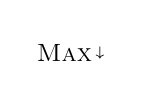
\begin{tikzpicture}[xscale=0.6,yscale=0.4]
\node (max) at (0,0) {{\small \textsc{Max}}};
\node (reg) at (0.75,0.5) {{\fns \textalpha}};
\node (arrow) at (0.75,0) {{\tiny $\downarrow$}};
\node (Rt) at (0.75,-0.5) {{\fns \textbeta}};
\end{tikzpicture}
\end{minipage}
}

\newcommand{\DepAB}{
\begin{minipage}{0.09\textwidth}
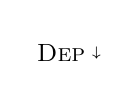
\begin{tikzpicture}[xscale=0.6,yscale=0.4]
\node (max) at (0,0) {{\small \textsc{Dep}}};
\node (reg) at (0.75,0.5) {{\fns \textalpha}};
\node (arrow) at (0.75,0) {{\tiny $\downarrow$}};
\node (Rt) at (0.75,-0.5) {{\fns \textbeta}};
\end{tikzpicture}
\end{minipage}
}

\newcommand{\DepHReg}{
\begin{minipage}{0.055\textwidth}
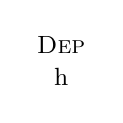
\begin{tikzpicture}[xscale=0.6,yscale=0.4]
\node (dep) at (0,0) {{\small \textsc{Dep}}};
\node (reg) at (0,-1.0) {{\small h}};
\end{tikzpicture}
\end{minipage}
}

\newcommand{\DepLReg}{
\begin{minipage}{0.055\textwidth}
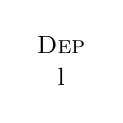
\begin{tikzpicture}[xscale=0.6,yscale=0.4]
\node (dep) at (0,0) {{\small \textsc{Dep}}};
\node (reg) at (0,-1.0) {{\small l}};
\end{tikzpicture}
\end{minipage}
}

\newcommand{\DepReg}{
\begin{minipage}{0.055\textwidth}
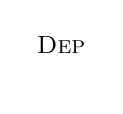
\begin{tikzpicture}[xscale=0.6,yscale=0.4]
\node (dep) at (0,0) {{\small \textsc{Dep}}};
\node (reg) at (0,-1.0) {{\small \textrho}};
\end{tikzpicture}
\end{minipage}
}

\newcommand{\DepTRt}{
\begin{minipage}{0.1\textwidth}
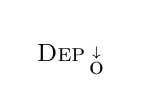
\begin{tikzpicture}[xscale=0.6,yscale=0.4]
\node (dep) at (0,0) {{\small \textsc{Dep}}};
\node (t) at (0.75,0.5) {{\fns \texttau}};
\node (arrow) at (0.75,0) {{\tiny $\downarrow$}};
\node (Rt) at (0.75,-0.5) {{\fns o}};
\end{tikzpicture}
\end{minipage}
}

\newcommand{\MaxRegRt}{
\begin{minipage}{0.1\textwidth}
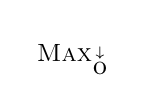
\begin{tikzpicture}[xscale=0.6,yscale=0.4]
\node (max) at (0,0) {{\small \textsc{Max}}};
\node (arrow) at (0.75,0) {{\tiny $\downarrow$}};
\node (Rt) at (0.75,-0.5) {{\fns o}};
\node (reg) at (0.75,0.5) {{\fns \textrho}};
\end{tikzpicture}
\end{minipage}
}

\newcommand{\RegToneByRt}{
\begin{minipage}{0.06\textwidth}
\begin{tikzpicture}[xscale=0.6,yscale=0.5]
\node[rotate=20] (arrow1) at (-0.15,0) {{\fns $\uparrow$}};
\node[rotate=340] (arrow2) at (0.15,0) {{\fns $\uparrow$}};
\node (Rt) at (0,-0.55) {{\small o}};
\node (reg) at (0.4,0.55) {{\small \textrho}};
\node (tone) at (-0.4,0.55) {{\small \texttau}};
\end{tikzpicture}
\end{minipage}
}

\newcommand{\RegToneBySyl}{
\begin{minipage}{0.06\textwidth}
\begin{tikzpicture}[xscale=0.6,yscale=0.5]
\node[rotate=20] (arrow1) at (-0.15,0) {{\fns $\uparrow$}};
\node[rotate=340] (arrow2) at (0.15,0) {{\fns $\uparrow$}};
\node (Rt) at (0,-0.55) {{\small \textsigma}};
\node (reg) at (0.4,0.55) {{\small \textrho}};
\node (tone) at (-0.4,0.55) {{\small \texttau}};
\end{tikzpicture}
\end{minipage}
}

\newcommand{\DepTone}{
\begin{minipage}{0.055\textwidth}
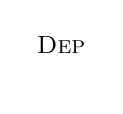
\begin{tikzpicture}[xscale=0.6,yscale=0.4]
\node (dep) at (0,0) {{\small \textsc{Dep}}};
\node (tone) at (0,-1.0) {{\small \texttau}};
\end{tikzpicture}
\end{minipage}
}

\newcommand{\DepTonalRt}{
\begin{minipage}{0.055\textwidth}
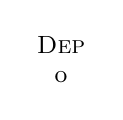
\begin{tikzpicture}[xscale=0.6,yscale=0.4]
\node (dep) at (0,0) {{\small \textsc{Dep}}};
\node (tone) at (0,-1.0) {{\small o}};
\end{tikzpicture}
\end{minipage}
}

\newcommand{\DepL}{
\begin{minipage}{0.055\textwidth}

\begin{tikzpicture}[xscale=0.6,yscale=0.4]
\node (dep) at (0,0) {{\small \textsc{Dep}}};
\node (tone) at (0,-1.0) {{\small L}};
\end{tikzpicture}
\end{minipage}
}

\newcommand{\DepH}{
\begin{minipage}{0.055\textwidth}

\begin{tikzpicture}[xscale=0.6,yscale=0.4]
\node (dep) at (0,0) {{\small \textsc{Dep}}};
\node (tone) at (0,-1.0) {{\small H}};
\end{tikzpicture}
\end{minipage}
}

\newcommand{\NoMultDiff}{{\small *loh}}
\newcommand{\Alt}{{\small \textsc{Alt}}}
\newcommand{\NoSkip}{{\small \scell{\textsc{No}\\\textsc{Skip}}}}


\newcommand{\RegDomRt}{
\begin{minipage}{0.030\textwidth}
\begin{tikzpicture}[xscale=0.6,yscale=0.5]
\node (arrow) at (0,0) {{\fns $\downarrow$}};
\node (Rt) at (0,-0.55) {{\small o}};
\node (reg) at (0,0.55) {{\small \textrho}};
\end{tikzpicture}
\end{minipage}
}

\newcommand{\DepRegRt}{
\begin{minipage}{0.1\textwidth}
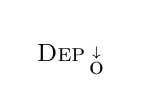
\begin{tikzpicture}[xscale=0.6,yscale=0.4]
\node (dep) at (0,0) {{\small \textsc{Dep}}};
\node (arrow) at (0.75,0) {{\tiny $\downarrow$}};
\node (Rt) at (0.75,-0.5) {{\fns o}};
\node (reg) at (0.75,0.5) {{\fns \textrho}};
\end{tikzpicture}
\end{minipage}
}

% unused

\newcommand{\ToneByRt}{
\begin{minipage}{0.05\textwidth}
\begin{tikzpicture}[xscale=0.6,yscale=0.5]
\node (arrow) at (0,0) {{\fns $\uparrow$}};
\node (Rt) at (0,-0.55) {{\small o}};
\node (tone) at (0,0.55) {{\small \texttau}};
\end{tikzpicture}
\end{minipage}
}

\newcommand{\RegByRt}{
\begin{minipage}{0.05\textwidth}
\begin{tikzpicture}[xscale=0.6,yscale=0.5]
\node (arrow) at (0,0) {{\fns $\uparrow$}};
\node (Rt) at (0,-0.55) {{\small o}};
\node (reg) at (0,0.55) {{\small \textrho}};
\end{tikzpicture}
\end{minipage}
}

\newcommand{\ToneDomRt}{
\begin{minipage}{0.05\textwidth}
\begin{tikzpicture}[xscale=0.6,yscale=0.5]
\node (arrow) at (0,0) {{\fns $\downarrow$}};
\node (Rt) at (0,-0.55) {{\small o}};
\node (tone) at (0,0.55) {{\small \texttau}};
\end{tikzpicture}
\end{minipage}
}

% --- OT tableaus --- %

% Sec. 3.2, first tabl.

\newcommand{\OTHLInput}{
\begin{minipage}{0.17\textwidth}
\begin{tikzpicture}[xscale=\myscalex,yscale=\myscaley]
\node (tone) at (2,0) {(= H)};
\node (syl) at (0,0) {\textsigma};
\node (Rt) at (0,1) {o};
\node (H) at (-0.5,2) {H};
\node (R) at (0.5,3) {h};
\node (Rt2) at (1.5,1.0) {o};
%\node (H2) at (1.0,2) {\epen{L}};
\node (R2) at (2.0,3) {\blue{l}};
\draw [thick] (syl.north) -- (Rt.south) ;
\draw [thick] (Rt.north) -- (H.south) ;
\draw [thick] (Rt.north) -- (R.south) ;
\draw [thick] (syl.north) -- (Rt2.south) ;
%\draw [dashed] (Rt2.north) -- (H2.south) ;
%\draw [dashed] (Rt2.north) -- (R2.south) ;
\end{tikzpicture}
\end{minipage}
}

\newcommand{\OTHLWinner}{
\begin{minipage}{0.17\textwidth}
\begin{tikzpicture}[xscale=\myscalex,yscale=\myscaley]
\node (tone) at (2,0) {(= HL)};
\node (syl) at (0,0) {\textsigma};
\node (Rt) at (0,1) {o};
\node (H) at (-0.5,2) {H};
\node (R) at (0.5,3) {h};
\node (Rt2) at (1.5,1.0) {o};
\node (H2) at (1.0,2) {\epen{L}};
\node (R2) at (2.0,3) {\blue{l}};
\draw [thick] (syl.north) -- (Rt.south) ;
\draw [thick] (Rt.north) -- (H.south) ;
\draw [thick] (Rt.north) -- (R.south) ;
\draw [thick] (syl.north) -- (Rt2.south) ;
\draw [dashed] (Rt2.north) -- (H2.south) ;
\draw [dashed] (Rt2.north) -- (R2.south) ;
\end{tikzpicture}
\end{minipage}
}

\newcommand{\OTHLSpreadingHOnly}{
\begin{minipage}{0.17\textwidth}
\begin{tikzpicture}[xscale=\myscalex,yscale=\myscaley]
\node (tone) at (2,0) {(= HM)};
\node (syl) at (0,0) {\textsigma};
\node (Rt) at (0,1) {o};
\node (H) at (-0.5,2) {H};
\node (R) at (0.5,3) {h};
\node (Rt2) at (1.5,1.0) {o};
%\node (H2) at (1.0,2) {\epen{L}};
\node (R2) at (2.0,3) {\blue{l}};
\draw [thick] (syl.north) -- (Rt.south) ;
\draw [thick] (Rt.north) -- (H.south) ;
\draw [thick] (Rt.north) -- (R.south) ;
\draw [thick] (syl.north) -- (Rt2.south) ;
\draw [dashed] (Rt2.north) -- (R2.south) ;
\draw [dashed] (Rt2.north) -- (H.south) ;
\end{tikzpicture}
\end{minipage}
}

\newcommand{\OTHLInsertH}{
\begin{minipage}{0.17\textwidth}
\begin{tikzpicture}[xscale=\myscalex,yscale=\myscaley]
\node (tone) at (2,0) {(= HM)};
\node (syl) at (0,0) {\textsigma};
\node (Rt) at (0,1) {o};
\node (H) at (-0.5,2) {H};
\node (R) at (0.5,3) {h};
\node (Rt2) at (1.5,1.0) {o};
\node (H2) at (1.0,2) {\epen{H}};
\node (R2) at (2.0,3) {\blue{l}};
\draw [thick] (syl.north) -- (Rt.south) ;
\draw [thick] (Rt.north) -- (H.south) ;
\draw [thick] (Rt.north) -- (R.south) ;
\draw [thick] (syl.north) -- (Rt2.south) ;
\draw [dashed] (Rt2.north) -- (H2.south) ;
\draw [dashed] (Rt2.north) -- (R2.south) ;
\end{tikzpicture}
\end{minipage}
}

\newcommand{\OTHLOverwriting}{
\begin{minipage}{0.17\textwidth}
\begin{tikzpicture}[xscale=\myscalex,yscale=\myscaley]
\node (syl) at (0,0) {\textsigma};
\node (Rt) at (0,1) {o};
\node (H) at (-0.5,2) {H};
\node (R) at (0.5,3) {h};
\node (Rt2) at (1.5,1.0) {o};
%\node (H2) at (1.0,2) {\epen{L}};
\node (R2) at (2.0,3) {\blue{l}};
\draw [thick] (syl.north) -- (Rt.south) ;
\draw [thick] (Rt.north) -- (H.south) ;
\draw [thick] (Rt.north) -- (R.south) ;
\draw [thick] (syl.north) -- (Rt2.south) ;
%\draw [dashed] (Rt2.north) -- (H2.south) ;
\draw [dashed] (Rt.north) -- (R2.south) ;
\node (del) at (0.3,1.9) {\textbf{=}};
\end{tikzpicture}
\end{minipage}
}

\newcommand{\OTHLSpreading}{
\begin{minipage}{0.17\textwidth}
\begin{tikzpicture}[xscale=\myscalex,yscale=\myscaley]
\node (syl) at (0,0) {\textsigma};
\node (Rt) at (0,1) {o};
\node (H) at (-0.5,2) {H};
\node (R) at (0.5,3) {h};
\node (Rt2) at (1.5,1.0) {o};
%\node (H2) at (1.0,2) {\epen{L}};
\node (R2) at (2.0,3) {\blue{l}};
\draw [thick] (syl.north) -- (Rt.south) ;
\draw [thick] (Rt.north) -- (H.south) ;
\draw [thick] (Rt.north) -- (R.south) ;
\draw [thick] (syl.north) -- (Rt2.south) ;
%\draw [dashed] (Rt2.north) -- (H2.south) ;
\draw [dashed] (Rt2.north) -- (H.south) ;
\draw [dashed] (Rt2.north) -- (R.south) ;
\end{tikzpicture}
\end{minipage}
}

% Sec. 4.2, second tabl.: phrase-medial position

\newcommand{\OTHnoLInput}{
\begin{minipage}{0.17\textwidth}
\begin{tikzpicture}[xscale=\myscalex,yscale=\myscaley]
\node (tone) at (2,0) {(= H)};
\node (syl) at (0,0) {\textsigma};
\node (Rt) at (0,1) {o};
\node (H) at (-0.5,2) {H};
\node (R) at (0.5,3) {h};
\node (Rt2) at (1.5,1.0) {o};
%\node (H2) at (1.0,2) {\epen{L}};
%\node (R2) at (2.0,3) {\blue{l}};
\draw [thick] (syl.north) -- (Rt.south) ;
\draw [thick] (Rt.north) -- (H.south) ;
\draw [thick] (Rt.north) -- (R.south) ;
\draw [thick] (syl.north) -- (Rt2.south) ;
\end{tikzpicture}
\end{minipage}
}

\newcommand{\OTHnoLEpenth}{
\begin{minipage}{0.17\textwidth}
\begin{tikzpicture}[xscale=\myscalex,yscale=\myscaley]
\node (tone) at (2,0) {(= HM)};
\node (syl) at (0,0) {\textsigma};
\node (Rt) at (0,1) {o};
\node (H) at (-0.5,2) {H};
\node (R) at (0.5,3) {h};
\node (Rt2) at (1.5,1.0) {o};
\node (H2) at (1.0,2) {\epen{L}};
\node (R2) at (2.0,3) {\epen{h}};
\draw [thick] (syl.north) -- (Rt.south) ;
\draw [thick] (Rt.north) -- (H.south) ;
\draw [thick] (Rt.north) -- (R.south) ;
\draw [thick] (syl.north) -- (Rt2.south) ;
\draw [dashed] (Rt2.north) -- (H2.south) ;
\draw [dashed] (Rt2.north) -- (R2.south) ;
\end{tikzpicture}
\end{minipage}
}

\newcommand{\OTHnoLSpreading}{
\begin{minipage}{0.17\textwidth}
\begin{tikzpicture}[xscale=\myscalex,yscale=\myscaley]
\node (tone) at (2,0) {(= HH)};
\node (syl) at (0,0) {\textsigma};
\node (Rt) at (0,1) {o};
\node (H) at (-0.5,2) {H};
\node (R) at (0.5,3) {h};
\node (Rt2) at (1.5,1.0) {o};
%\node (H2) at (1.0,2) {\epen{L}};
%\node (R2) at (2.0,3) {\blue{l}};
\draw [thick] (syl.north) -- (Rt.south) ;
\draw [thick] (Rt.north) -- (H.south) ;
\draw [thick] (Rt.north) -- (R.south) ;
\draw [thick] (syl.north) -- (Rt2.south) ;
\draw [dashed] (Rt2.north) -- (H.south) ;
\draw [dashed] (Rt2.north) -- (R.south) ;
\end{tikzpicture}
\end{minipage}
}

% Sec. 4.2, third tabl., LM is unaffected by L\%

\newcommand{\OTLMInput}{
\begin{minipage}{0.2\textwidth}
\begin{tikzpicture}[xscale=\myscalex,yscale=\myscaley]
\node (tone) at (2,0) {(= LM)};
\node (syl) at (0,0) {\textsigma};
\node (Rt) at (0,1) {o};
\node (H) at (-0.5,2) {L};
\node (R) at (0.5,3) {l};
\node (Rt2) at (1.5,1.0) {o};
\node (H2) at (1.0,2) {L};
\node (R2) at (2.0,3) {h};
\node (R3) at (3.0,3) {\blue{l}};
\draw [thick] (syl.north) -- (Rt.south) ;
\draw [thick] (Rt.north) -- (H.south) ;
\draw [thick] (Rt.north) -- (R.south) ;
\draw [thick] (syl.north) -- (Rt2.south) ;
\draw [thick] (Rt2.north) -- (H2.south) ;
\draw [thick] (Rt2.north) -- (R2.south) ;
\end{tikzpicture}
\end{minipage}
}

\newcommand{\OTLMReplace}{
\begin{minipage}{0.2\textwidth}
\begin{tikzpicture}[xscale=\myscalex,yscale=\myscaley]
\node (tone) at (2,0) {(= LL)};
\node (syl) at (0,0) {\textsigma};
\node (Rt) at (0,1) {o};
\node (H) at (-0.5,2) {L};
\node (R) at (0.5,3) {l};
\node (Rt2) at (1.5,1.0) {o};
\node (H2) at (1.0,2) {L};
\node (R2) at (2.0,3) {h};
\node (R3) at (3.0,3) {\blue{l}};
\draw [thick] (syl.north) -- (Rt.south) ;
\draw [thick] (Rt.north) -- (H.south) ;
\draw [thick] (Rt.north) -- (R.south) ;
\draw [thick] (syl.north) -- (Rt2.south) ;
\draw [thick] (Rt2.north) -- (H2.south) ;
\draw [thick] (Rt2.north) -- (R2.south) ;
\draw [dashed] (Rt2.north) -- (R3.south) ;
\node (del) at (1.8,2.1) {\textbf{=}};
\end{tikzpicture}
\end{minipage}
}

\newcommand{\OTLMTwoReg}{
\begin{minipage}{0.2\textwidth}
\begin{tikzpicture}[xscale=\myscalex,yscale=\myscaley]
\node (tone) at (2,0) {(= LML)};
\node (syl) at (0,0) {\textsigma};
\node (Rt) at (0,1) {o};
\node (H) at (-0.5,2) {L};
\node (R) at (0.5,3) {l};
\node (Rt2) at (1.5,1.0) {o};
\node (H2) at (1.0,2) {L};
\node (R2) at (2.0,3) {h};
\node (R3) at (3.0,3) {\blue{l}};
\draw [thick] (syl.north) -- (Rt.south) ;
\draw [thick] (Rt.north) -- (H.south) ;
\draw [thick] (Rt.north) -- (R.south) ;
\draw [thick] (syl.north) -- (Rt2.south) ;
\draw [thick] (Rt2.north) -- (H2.south) ;
\draw [thick] (Rt2.north) -- (R2.south) ;
\draw [dashed] (Rt2.north) -- (R3.south) ;
\end{tikzpicture}
\end{minipage}
}

% Sec. 4.2, fourth tabl., L is affected by L\% but M is not

\newcommand{\OTLInput}{
\begin{minipage}{0.17\textwidth}
\begin{tikzpicture}[xscale=\myscalex,yscale=\myscaley]
\node (tone) at (2,0) {(= L)};
\node (syl) at (0,0) {\textsigma};
\node (Rt) at (0,1) {o};
\node (H) at (-0.5,2) {L};
\node (R) at (0.5,3) {l};
\node (R2) at (2,3) {\blue{l}};
\draw [thick] (syl.north) -- (Rt.south) ;
\draw [thick] (Rt.north) -- (H.south) ;
\draw [thick] (Rt.north) -- (R.south) ;
\end{tikzpicture}
\end{minipage}
}

\newcommand{\OTLLowered}{
\begin{minipage}{0.17\textwidth}
\begin{tikzpicture}[xscale=\myscalex,yscale=\myscaley]
\node (tone) at (2,0) {(= LL)};
\node (syl) at (0,0) {\textsigma};
\node (Rt) at (0,1) {o};
\node (H) at (-0.5,2) {L};
\node (R) at (0.5,3) {l};
\node (R2) at (2,3) {\blue{l}};
\draw [thick] (syl.north) -- (Rt.south) ;
\draw [thick] (Rt.north) -- (H.south) ;
\draw [thick] (Rt.north) -- (R.south) ;
\draw [dashed] (Rt.north) -- (R2.south) ;
\end{tikzpicture}
\end{minipage}
}

\newcommand{\OTMInput}{
\begin{minipage}{0.17\textwidth}
\begin{tikzpicture}[xscale=\myscalex,yscale=\myscaley]
\node (tone) at (2,0) {(= M)};
\node (syl) at (0,0) {\textsigma};
\node (Rt) at (0,1) {o};
\node (H) at (-0.5,2) {L};
\node (R) at (0.5,3) {h};
\node (R2) at (2,3) {\blue{l}};
\draw [thick] (syl.north) -- (Rt.south) ;
\draw [thick] (Rt.north) -- (H.south) ;
\draw [thick] (Rt.north) -- (R.south) ;
\end{tikzpicture}
\end{minipage}
}

\newcommand{\OTMLowered}{
\begin{minipage}{0.17\textwidth}
\begin{tikzpicture}[xscale=\myscalex,yscale=\myscaley]
\node (tone) at (2,0) {(= ML)};
\node (syl) at (0,0) {\textsigma};
\node (Rt) at (0,1) {o};
\node (H) at (-0.5,2) {L};
\node (R) at (0.5,3) {h};
\node (R2) at (2,3) {\blue{l}};
\draw [thick] (syl.north) -- (Rt.south) ;
\draw [thick] (Rt.north) -- (H.south) ;
\draw [thick] (Rt.north) -- (R.south) ;
\draw [dashed] (Rt.north) -- (R2.south) ;
\end{tikzpicture}
\end{minipage}
}

% Sec. 4.2, fifth tableau, polar questions with level tones

\newcommand{\OTLPolIn}{
\begin{minipage}{0.20\textwidth}
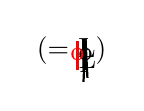
\begin{tikzpicture}[xscale=\myscalex-0.05,yscale=\myscaley-0.05]
\node (tone) at (3.5,0) {(= L)};
\node (syl) at (0,0) {\textsigma};
\node (syl2) at (2,0) {\red{\textsigma}};
\node (Rt) at (0,1) {o};
\node (H) at (-0.5,2) {L};
\node (R) at (0.5,3) {l};
\node (Rt2) at (2,1) {\red{o}};
\draw [thick] (syl.north) -- (Rt.south) ;
\draw [thick,red] (syl2.north) -- (Rt2.south) ;
\draw [thick] (Rt.north) -- (H.south) ;
\draw [thick] (Rt.north) -- (R.south) ;
\end{tikzpicture}
\end{minipage}
}

\newcommand{\OTLPolDef}{
\begin{minipage}{0.20\textwidth}
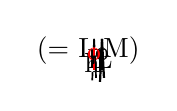
\begin{tikzpicture}[xscale=\myscalex-0.05,yscale=\myscaley-0.05]
\node (tone) at (3.5,0) {(= L.M)};
\node (syl) at (0,0) {\textsigma};
\node (syl2) at (2,0) {\red{\textsigma}};
\node (Rt) at (0,1) {o};
\node (H) at (-0.5,2) {L};
\node (R) at (0.5,3) {l};
\node (H2) at (1.5,2) {\epen{L}};
\node (R2) at (2.5,3) {\epen{h}};
\node (Rt2) at (2,1) {\red{o}};
\draw [thick] (syl.north) -- (Rt.south) ;
\draw [thick,red] (syl2.north) -- (Rt2.south) ;
\draw [thick] (Rt.north) -- (H.south) ;
\draw [thick] (Rt.north) -- (R.south) ;
\draw [semithick,dashed] (Rt2.north) -- (H2.south) ;
\draw [semithick,dashed] (Rt2.north) -- (R2.south) ;
\end{tikzpicture}
\end{minipage}
}

\newcommand{\OTLPolAlt}{
\begin{minipage}{0.20\textwidth}
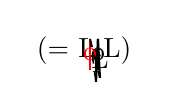
\begin{tikzpicture}[xscale=\myscalex-0.05,yscale=\myscaley-0.05]
\node (tone) at (3.5,0) {(= L.L)};
\node (syl) at (0,0) {\textsigma};
\node (syl2) at (2,0) {\red{\textsigma}};
\node (Rt) at (0,1) {o};
\node (H) at (-0.5,2) {L};
\node (R) at (0.5,3) {l};
\node (Rt2) at (2,1) {\red{o}};
\draw [thick] (syl.north) -- (Rt.south) ;
\draw [thick,red] (syl2.north) -- (Rt2.south) ;
\draw [thick] (Rt.north) -- (H.south) ;
\draw [thick] (Rt.north) -- (R.south) ;
\draw [semithick,dashed] (Rt2.north) -- (H.south) ;
\draw [semithick,dashed] (Rt2.north) -- (R.south) ;
\end{tikzpicture}
\end{minipage}
}

% Sec. 4.2, sixth tableau, polar questions with contour tones

\newcommand{\OTLLPolIn}{
\begin{minipage}{0.23\textwidth}
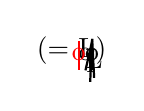
\begin{tikzpicture}[xscale=\myscalex-0.05,yscale=\myscaley-0.05]
\node (tone) at (5.2,0) {(= L)};
\node (syl) at (0,0) {\textsigma};
\node (syl3) at (3.4,0) {\red{\textsigma}};
\node (Rt) at (0,1) {o};
\node (Rt2) at (1.7,1) {o};
\node (Rt3) at (3.4,1) {\red{o}};
\node (H) at (-0.5,2) {L};
\node (R) at (0.5,3) {l};
\draw [thick] (syl.north) -- (Rt.south) ;
\draw [thick] (syl.north) -- (Rt2.south) ;
\draw [thick,red] (syl3.north) -- (Rt3.south) ;
\draw [thick] (Rt.north) -- (H.south) ;
\draw [thick] (Rt.north) -- (R.south) ;
\end{tikzpicture}
\end{minipage}
}

\newcommand{\OTLLPolDef}{
\begin{minipage}{0.23\textwidth}
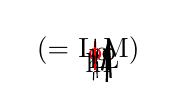
\begin{tikzpicture}[xscale=\myscalex-0.05,yscale=\myscaley-0.05]
\node (tone) at (5.2,0) {(= L.M)};
\node (syl) at (0,0) {\textsigma};
\node (syl3) at (3.4,0) {\red{\textsigma}};
\node (Rt) at (0,1) {o};
\node (Rt2) at (1.7,1) {o};
\node (Rt3) at (3.4,1) {\red{o}};
\node (H) at (-0.5,2) {L};
\node (R) at (0.5,3) {l};
\node (H3) at (2.9,2) {\epen{L}};
\node (R3) at (3.9,3) {\epen{h}};
\draw [thick] (syl.north) -- (Rt.south) ;
\draw [thick] (syl.north) -- (Rt2.south) ;
\draw [thick,red] (syl3.north) -- (Rt3.south) ;
\draw [thick] (Rt.north) -- (H.south) ;
\draw [thick] (Rt.north) -- (R.south) ;
\draw [dashed] (Rt3.north) -- (H3.south) ;
\draw [dashed] (Rt3.north) -- (R3.south) ;
\end{tikzpicture}
\end{minipage}
}

\newcommand{\OTLLPolSkip}{
\begin{minipage}{0.23\textwidth}
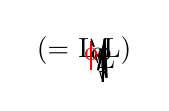
\begin{tikzpicture}[xscale=\myscalex-0.05,yscale=\myscaley-0.05]
\node (tone) at (5.2,0) {(= L.L)};
\node (syl) at (0,0) {\textsigma};
\node (syl3) at (3.4,0) {\red{\textsigma}};
\node (Rt) at (0,1) {o};
\node (Rt2) at (1.7,1) {o};
\node (Rt3) at (3.4,1) {\red{o}};
\node (H) at (-0.5,2) {L};
\node (R) at (0.5,3) {l};
\draw [thick] (syl.north) -- (Rt.south) ;
\draw [thick] (syl.north) -- (Rt2.south) ;
\draw [thick,red] (syl3.north) -- (Rt3.south) ;
\draw [thick] (Rt.north) -- (H.south) ;
\draw [thick] (Rt.north) -- (R.south) ;
\draw [dashed] (Rt3.north) -- (H.south) ;
\draw [dashed] (Rt3.north) -- (R.south) ;
\end{tikzpicture}
\end{minipage}
}  
  
\newcommand{\ilit}[1]{#1\il{#1}}    
\newcommand{\isit}[1]{#1\is{#1}}  

\makeatletter
\let\thetitle\@title
\let\theauthor\@author 
\makeatother

\newcommand{\togglepaper}[1][0]{ 
  \bibliography{../localbibliography}
  %% hyphenation points for line breaks
%% Normally, automatic hyphenation in LaTeX is very good
%% If a word is mis-hyphenated, add it to this file
%%
%% add information to TeX file before \begin{document} with:
%% %% hyphenation points for line breaks
%% Normally, automatic hyphenation in LaTeX is very good
%% If a word is mis-hyphenated, add it to this file
%%
%% add information to TeX file before \begin{document} with:
%% \include{localhyphenation}
\hyphenation{
affri-ca-te
affri-ca-tes
com-ple-ments
par-a-digm
Sha-ron
Kings-ton
phe-nom-e-non
Daul-ton
Abu-ba-ka-ri
Ngo-nya-ni
Clem-ents 
King-ston
Tru-cken-brodt
Tab-leau
cophono-logies
mark-edness
Ti-gri-nya
a-mong
Car-stens
Lu-bu-ku-su
}
\hyphenation{
affri-ca-te
affri-ca-tes
com-ple-ments
par-a-digm
Sha-ron
Kings-ton
phe-nom-e-non
Daul-ton
Abu-ba-ka-ri
Ngo-nya-ni
Clem-ents 
King-ston
Tru-cken-brodt
Tab-leau
cophono-logies
mark-edness
Ti-gri-nya
a-mong
Car-stens
Lu-bu-ku-su
}
  \papernote{\scriptsize\normalfont
    \theauthor.
    \thetitle. 
    To appear in: 
    Emily Clem,   Peter Jenks \& Hannah Sande.
    Theory and description in African Linguistics: Selected papers from the 47th Annual Conference on African Linguistics.
    Berlin: Language Science Press. [preliminary page numbering]
  }
  \pagenumbering{roman}
  \setcounter{chapter}{#1}
  \addtocounter{chapter}{-1}
}

\newcommand{\upstep}{\textupstep}


% \newcounter{tableauxcounter}

\renewcommand{\textltailn}{ɲ}
\renewcommand{\textbardotlessj}{ɟ}

\newcommand{\emphkh}[1]{\textit{#1}} %originally \textbf, banned by the guidelines



\definecolor{lsDOIGray}{cmyk}{0,0,0,0.45}


\newcommand{\xuparrow}[1]{%
  {\left\uparrow\vbox to #1{}\right.\kern-\nulldelimiterspace}
}
\renewcommand \textupstep[1]{\char"A71B#1}
\renewcommand \textdownstep[1]{\char"A71C#1}
 
 \newcommand{\ꜛ}{\textsf{ꜛ}}
 
\def\biberror{\undefined}


\newcommand{\OTbox}[1]{\resizebox{.88\textwidth}{!}{#1}}
 
\usepackage{pifont.sty}

\author{Hasiyatu Abubakari\affiliation{University of Vienna, Austria}}
\title{Contrastive focus particles in Kʋ́sáàl} 


\abstract{This paper presents and discusses the particles used in expressing contrastive focus\footnote{The use of the term contrastive focus is aligned with what \citet{ÉKiss1998} refers to as exhaustive focus or identificational focus. With this background, the terminological use of identificational focus, contrastive focus and exhaustive focus are meant to refer to the same notion that is expressed by the particles \textit{kà, ń, nɛ́} in Kʋ́sáàl.} in Kʋ́sáàl, a Gur language spoken in Ghana, Burkina Faso and Togo. Contrary to the earlier claim made by \citet{Abubakari2011} that focus is morphologically null in the language, the particles \textit{kà}, \textit{ń} and \textit{nɛ́} are identified as contrastive focus markers in Kʋ́sáàl. The particle \textit{kà} is limited to fronted focused items, whilst \textit{ń} and \textit{nɛ́} are limited to in-situ focused constituents. Ex-situ focus always bears contrastive interpretation, hence the obligatory use of \textit{kà}. In-situ focus is marked prosodically. However, the in-situ use of \textit{ń} and \textit{nɛ́} correlates with a contrastive and exhaustive focus interpretation. To determine the validity of \textit{ń, nɛ́} and \textit{kà} as contrastive focus particles, I subject them to various tests of exhaustivity from which I conclude that these are contrastive focus particles in the language.}

%Key words: Kʋsaal, focus particles, contrastive/exhaustive focus, information focus

\begin{document}

\maketitle

% \section{Introduction}
% <<<<<<< HEAD
% % \todo[inline]{check the paper for ʋ and $\upsilon$ and unify if appropriate}
% The concept of contrastive \isi{focus}, marked with different strategies in most languages, has received a lot of attention in the literature. \citet{ÉKiss1998} looks at the concept with data from \ili{Hungarian} and \ili{English}, \citet{horn1981} with data from \ili{English}, \citet{szabolcsi1981} with \ili{Hungarian}, \citet{hartmann2007} with \ili{Hausa}, and \citet{duah2015} with \ili{Akan}. Additionally, \citet{hudu2012} discusses contrastive \isi{focus} constructions in \ili{Dagbani}, \citet{hiraiwa2005} and \citet{hiraiwabodomo2008} also mention \isi{focus} constructions in \ili{Buli} and \ili{Dagaare} respectively. \citet{Abubakari2011} analyses \isi{focus} as morphologically null in Kʋsáàl. This paper seeks to clarify that notion by showing that \textit{information} \isi{focus} is not overtly marked since Kʋsáàl does not have a grammatical \isi{focus} marker (\ref{ex:abubakari:1}b); but \textit{contrastive} \isi{focus} is marked using the particles \textit{kà, ń, nɛ} (\ref{ex:abubakari:2}a-b). 
% =======
% \todo[inline]{check the paper for ʋ and $\upsilon$ and unify if appropriate}
The concept of contrastive \isi{focus}, marked with different strategies in most languages, has received a lot of attention in the literature. \citet{ÉKiss1998} looks at the concept with data from \ili{Hungarian} and \ili{English}, \citet{horn1981} with data from \ili{English}, \citet{szabolcsi1981} with \ili{Hungarian}, \citet{hartmann2007} with \ili{Hausa}, and \citet{duah2015} with \ili{Akan}. Additionally, \citet{hudu2012} discusses contrastive \isi{focus} constructions in \ili{Dagbani}, \citet{hiraiwa2005} and \citet{hiraiwabodomo2008} also mention \isi{focus} constructions in \ili{Buli} and \ili{Dagaare} respectively. \citet{Abubakari2011} analyses \isi{focus} as morphologically null in Kʋ́sáàl. This paper seeks to clarify that notion by showing that \textit{information} \isi{focus} is not overtly marked since Kʋ́sáàl does not have a grammatical \isi{focus} marker (\ref{ex:abubakari:1}b); but \textit{contrastive} \isi{focus} is marked using the particles \textit{kà, ń, nɛ́} (\ref{ex:abubakari:2}a-b). 
% >>>>>>> e0241a6872529cc2f2761cad2f0e5b047737d375

Context: Meals are not to be repeated; the questioner in (\ref{ex:abubakari:1}a) knows that the children ate something yesterday but does not know what exactly they ate. Focus is therefore on what was eaten.\footnote{Verbs do not inflect for tense in Kʋ́sáàl. The remoteness of an activity is expressed using particles. The particle \textit{sà} means the event is a day old, \textit{dàà} means the event is two days old but less than a year and \textit{dà} means the event is a year and beyond.}

% TODO Ask about the footnote
 
\ea\label{ex:abubakari:1}
\ea\label{ex:abubakari:1a}
Q: \gll Bíís    lá  sà dī    bɔ́?\\                 
children  \textsc{def}  \textsc{prt}  eat.\textsc{perf}  what\\                     
\glt ‘What did the children eat yesterday?’    

\ex\label{ex:abubakari:1b}
Ans: \gll Bíís    lá  sà  dī \textbf{\textit{mùì}}.\\
children    \textsc{def}  \textsc{prt}  eat.\textsc{perf}  rice\\
\glt ‘The children eat \textit{rice} yesterday.’  
 \z
 \z
 
Context: The hearer thought the children ate something other than rice, for example beans. The sentences in (\ref{ex:abubakari:2}a-b) are corrections to the perceived notion of what was eaten yesterday. 
 
 
\ea\label{ex:abubakari:2}
\ea\label{ex:abubakari:2a}
\gll \textbf{\textit{Mùì} }kà  bà  sá  dī.  \\ 
rice  \textsc{foc}  3\textsc{pl}.  \textsc{prt}  eat.\textsc{perf}   \\                  
\glt ‘It is \textit{rice} (and nothing else) that they ate yesterday’    

\ex\label{ex:abubakari:2b}
\gll Bà  sà  dī    nɛ́ \textbf{\textit{mùì.}}\\
3\textsc{pl}.  \textsc{prt}  eat.\textsc{perf}  \textsc{foc}  rice\\
\glt ‘It is \textit{rice} (and nothing else) that they ate yesterday’
\z
\z

In these examples, (\ref{ex:abubakari:1}b) is an instance of information or presentational \isi{focus}, where the focused constituent does not carry any \isi{contrastive interpretation}. The utterances in (\ref{ex:abubakari:2}a-b) on the other hand convey exhaustive interpretation, where what is eaten is not only emphasized but also exhaustive (in the sense that \textit{only rice} is eaten) and contrastive (in the sense that \textit{what is eaten is rice and nothing else}). 

Extensive research on discourse-related information widely differentiates between two different forms of \isi{focus} \citep{Halliday1967, chafe1976,szabolcsi1981,michael1986,ÉKiss1998,Vallduví1998,Molnár2002}. \citet{ÉKiss1998} refers to the two forms as: “\isi{information focus}” and  “\isi{identificational focus}”. Alongside \citet{ÉKiss1998}, \citet{Vallduví1998} and \citet{selkirk2008}, where it is assumed that the evocation of alternative is restricted to contrastive or \isi{identificational focus}, another widely acknowledged semantic definition of \isi{focus} is \citeauthor{rooth1985}’s (\citeyear{rooth1985}; \citeyear{Rooth1992}; \citeyear{rooth1996}) “alternative semantics” where the argument is made that “\isi{focus} indicates the presence of alternatives that are relevant for the interpretation of linguistic expression” (cf \citealt{krifka2007}:6).  By consequence, any kind of \isi{focus} is assumed to set an alternative against which focused constituents are evaluated. This line of argumentation is followed by Zimmermann, who further adds that: 

\begin{quote}
…the alternatives that play a role with contrastive \isi{focus} are not just calculated relative to the semantic denotation of the \isi{focus} constituent (the semantic alternative). Instead, they are calculated relative to the \isi{focus} denotation together with the speaker’s suppositions as to which of these alternatives the hearer is likely to expect (discourse-semantic alternative). \citep[3]{Zimmermann2008}. 
\end{quote}

This work is not intended to go through the merits or demerits of these arguments. The fundamental goal is to provide empirical evidence in support of the claim that Kʋ́sáàl does not have an overt grammatical \isi{focus particle} and that the particles \textit{kà, ń} and \textit{nɛ́} are used in marking contrastive \isi{focus}. I will therefore align this work with the definition of \citet{ÉKiss1998}, which provides the platform for differentiating \isi{information focus}, which is morphologically null, from \isi{identificational focus}, which uses the particles \textit{kà, ń} and \textit{nɛ́} in Kʋ́sáàl. The following serve as the working definitions for (I) \isi{information focus} and (II) \isi{identificational focus} respectively. 

\begin{enumerate}
	\item[(I)]  ‘‘If a sentence part conveys new, nonpresupposed information marked by one or more pitch accents – without expressing exhaustive identification performed on a set of contextually or situationally given entities, it is a mere \isi{information focus}.”  \citep[246]{ÉKiss1998}
 

 
	\item[(II)]  ‘‘An \isi{identificational focus} represents a subset of the set of contextually or situationally given elements for which the predicate phrase can potentially hold; it is identified as the exhaustive subset of this set for which the predicate phrase actually holds.” \citep[249]{ÉKiss1998}
\end{enumerate}  

In this paper I discuss the syntax and semantics of the particles \textit{kà, ń,} and \textit{nɛ́} in Kʋ́sáàl and argue that these particles are used in expressing exhaustive/contrastive \isi{focus} every time they occur in a construction with \isi{focus} interpretation. Whereas the particle \textit{kà} is limited to fronted focused items only and is obligatory whenever fronting occurs, \textit{ń} and \textit{nɛ́} are limited to in-situ focused constituents any time a contrastive/exhaustive \isi{focus} interpretation is desired. Ex-situ \isi{focus} always bears a \isi{contrastive interpretation} and as such requires the obligatory use of \textit{kà}. Kʋ́sáàl marks \isi{in-situ focus} using focal stress. The use of \textit{ń} and \textit{nɛ́} correlates with a contrastive/exhaustive \isi{focus} interpretation. The grounds for these assertions are born out of the observed syntactic and semantic properties exhibited by these particles in Kʋ́sáàl. Even though they perform similar functions compared to grammatical \isi{focus} markers by triggering \isi{focus} related interpretations, they differ significantly from default grammatical \isi{focus} markers on the following grounds: First, the particles \textit{kà}, \textit{ń} and \textit{nɛ́} are not default grammatical \isi{focus} elements like \textit{lá} and its variants in \ili{Dagaare}, where the default \isi{focus} marker must obligatorily occur in all declarative constructions \citep{Bodomo1997}, even when no contrastive/exhaustive \isi{focus} interpretations are encoded. Second, the presence of these particles has a direct semantic impact on the interpretation of the focused constituent. Either they cause an exhaustive/\isi{contrastive interpretation} of the focused item, or the focused status of the constituent could be said to cause the appearance of these particles. They are excluded in non-exhaustive environments such as ‘mention-some’ contexts or contexts where a property is known to hold more than the focused entity \citep[242]{hartmann2007}. 

Some of the major questions this paper seeks to answer are:
(1) How is discourse-related information packaged using the particles \textit{kà, ń} and \textit{nɛ́} in Kʋ́sáàl? 
(2) How can one determine whether indeed the identified particles are contrastive/exhaustive \isi{focus} particles in Kʋ́sáàl? 

The paper is organized into five sections. The second section looks at information packaging strategies in Kʋ́sáàl and analyses the various types of \isi{focus} constructions. In the third and fourth sections, I apply various standard tests for exhaustivity on the identified \isi{focus} particles to verify whether they are indeed contrastive/exhaustive \isi{focus} particles. The conclusion forms the final section.

\section{Focus constructions in Kʋ́sáàl}

As indicated earlier, this work uses the definition of \citet{ÉKiss1998} as a background in analyzing and setting apart the two types of \isi{focus} in Kʋ́sáàl. Information or presentational \isi{focus} is expressed prosodically where the focused item receives extra stress in its pronunciation. No grammaticalized \isi{focus particle} is used in such instances. Information \isi{focus} is therefore argued to be overtly null in Kʋ́sáàl. Contrastive \isi{focus} on the other hand uses the particles \textit{kà, ń,} and \textit{nɛ́}. In the following subsections, I present various contexts that naturally elucidate the use of \isi{information focus} (\sectref{sec:abubakari:2.1}) and contrastive \isi{focus} (\sectref{sec:abubakari:2.2}).

\subsection{Information focus constructions in Kʋ́sáàl}\label{sec:abubakari:2.1}

% <<<<<<< HEAD
% Following the definition in (I) by \citet[246]{ÉKiss1998}, the notions expressed using \isi{information focus} are not expected to be exhaustive in nature. They serve to dissuade one’s ignorance about an event, action or situation. The answers to the \textit{wh}-questions in the examples below represent instances of \isi{information focus} in Kʋsáàl. 
% =======
Following the definition in (I) by \citet[246]{ÉKiss1998}, the notions expressed using \isi{information focus} are not expected to be exhaustive in nature. They serve to dissuade one’s ignorance about an event, action or situation. The answers to the \textit{wh}{}-questions in the examples below represent instances of \isi{information focus} in Kʋ́sáàl. 
% >>>>>>> e0241a6872529cc2f2761cad2f0e5b047737d375

Context 1: Several things need to be done. The questioner does not know the activity carried out by a partner and underrates the relevance of what was done. The question in (\ref{ex:abubakari:3}a) is used and the response in (\ref{ex:abubakari:3}b) provides new information with \isi{focus} on the activity that was carried out. It could be that several other activities were carried out but the most salient is the \textit{buying of the items}
 
\ea\label{ex:abubakari:3}
\ea{ \label{ex:abubakari:3a}
Q: \gll \`{O}    sà  k\={e}ŋŋɛ̄    māāl    bɔ́?         \\
3Sg  \textsc{prt}  go.\textsc{perf}  do.\textsc{perf}  what\\}
\glt ‘What at all did s/she go to do yesterday.’   
\ex{ \label{ex:abubakari:3b}
Ans: \gll \`{O}  sà  k\={e}ŋŋɛ̄ \textbf{\textit{dāˈ}}    \textbf{\textit{láˈád} } \textbf{\textit{lá.}}\\
3\textsc{sg}  \textsc{prt}  go.\textsc{perf}  buy.\textsc{perf}  items
 \textsc{def}\\}
\glt ‘S/he went and \textit{bought the items} yesterday.’
 \z
 \z
 
Context 2: A group of children are playing. The youngest one is hit and he starts crying. The mother in (\ref{ex:abubakari:4}a) wants to know who hit the child. One of the children who saw \textit{Aduku} hitting the child responds as in (\ref{ex:abubakari:4}b). It could also be the case that there are other children who hit the child although they are not mentioned. 
 
\ea\label{ex:abubakari:4}
\ea{ \label{ex:abubakari:4a}
Q: \gll Ànɔ́’ɔn  bʋ̄ˈ    bííg  lá?\\ 
who    beat-\textsc{perf}  child  \textsc{def}. \\}                         
\glt ‘Who beat the child?’ 
\ex{\label{ex:abubakari:4b}
Ans: \gll \textbf{\textit{Àdúkú} } bʋ̄ˈ    bííg  lá.\\
Aduku  beat-\textsc{perf}  child  \textsc{def}.\\}
\glt ‘\textit{Aduku} beat the child.’\\
\z
\z
\textit{Aduku}’s mother also hears that her child has beaten someone, and asks to know who her child has beaten (\ref{ex:abubakari:5}a). Again it could be that there are other victims of \textit{Aduku} but only \textit{Asibi} is mentioned (\ref{ex:abubakari:5}b).

 
 
\ea\label{ex:abubakari:5}
\ea{ \label{ex:abubakari:5a}
Q: \gll Àdúkú  bʋˈ    ànɔ́ˈɔ́nɛ́?          \\
Aduku  beat-\textsc{perf}  who \\                          
}
\glt ‘Who did Aduku beat?’ 
\ex{ \label{ex:abubakari:5b}
Ans: \gll Àdúkú    bʋ̄ˈ \textbf{\textit{Àsíbí.}}    \\
Aduku    beat-\textsc{perf}  Asibi.\\
}
\glt ‘Aduku beat \textit{Asibi}.    
\z
\z

In all the answers to questions (\ref{ex:abubakari:3}a-\ref{ex:abubakari:5}i) above, the sentences convey new, nonpresupposed information, since the questioner has no knowledge of the information or the response the respondent is going to offer. The focused items do not have any form of contrastive/exhaustive interpretation and no overt morphological \isi{focus} particles are used. 

\subsection{Contrastive focus constructions in Kʋ́sáàl}\label{sec:abubakari:2.2}

Again following the working definition for \isi{identificational focus} in (II), it will be seen that unlike \isi{information focus}, contrastive \isi{focus} constructions are largely inherently exhaustive or exhaustive by implicature. I illustrate the various distributions of the particles \textit{kà, ń, nɛ́} in packaging this notion.

\subsubsection{Ex-situ focus marking with \textit{kà}}

% <<<<<<< HEAD
% The particle \textit{kà} occurs immediately after any item fronted to the left periphery of any construction. \textit{Wh}-\isi{focus} phrases are assumed to have moved to a designated \isi{focus} position and they co-occur with the ex-situ \isi{focus particle} \textit{kà} (see \citealt{aboh2007}). Answers to questions involving \textit{wh}-focus-phrases must have the particle \textit{kà} after the focused constituent. It is ungrammatical to substitute \textit{kà} with either \textit{ń} or \textit{nɛ} in ex-situ \isi{focus} constructions in the language. 
% =======
The particle \textit{kà} occurs immediately after any item fronted to the left periphery of any construction. \textit{Wh}{}-\isi{focus} phrases are assumed to have moved to a designated \isi{focus} position and they co-occur with the ex-situ \isi{focus particle} \textit{kà} (see \citealt{aboh2007}). Answers to questions involving \textit{wh}{}-focus-phrases must have the particle \textit{kà} after the focused constituent. It is ungrammatical to substitute \textit{kà} with either \textit{ń} or \textit{nɛ́} in ex-situ \isi{focus} constructions in the language. 
% >>>>>>> e0241a6872529cc2f2761cad2f0e5b047737d375

 
\ea\label{ex:abubakari:6}
\ea \label{ex:abubakari:6a} 
Q:\gll Bɔ́  kà  fʋ̀  dá  dāˈ:    bʋ́ʋ́g  bɛ́ɛ  \textit{pɛ́ˈʋ́gɔ́?}\\  
what  \textsc{foc}  2\textsc{sg}  \textsc{prt}  buy.\textsc{perf}:  goat  or 
sheep          \\
\glt ‘What did you buy: a goat or a sheep?’ 

\ex \label{ex:abubakari:6b} 
Q: \gll *Bɔ́  nɛ́  fʋ̀  dá  dāˈ:    bʋ́ʋ́g  bɛ́ɛ \textit{pɛ́ˈʋ́gɔ́?}\\
 what  \textsc{foc}  2\textsc{sg}  \textsc{prt}  buy.\textsc{perf}:  goat  or  sheep\\
  
\glt ‘What did you buy: a goat or a sheep?’ 

\ex \label{ex:abubakari:6c}
Q: \gll *Bɔ́  ń  fʋ  dá  dāˈ:    bʋ́ʋ́g  bɛ́ɛ \textit{pɛ́ˈʋ́gɔ́?}\\
what  \textsc{foc}  2\textsc{sg}  \textsc{prt}  buy.\textsc{perf}:  goat  or sheep \\
\glt ‘What did you buy: a goat or a sheep?’ 

\ex \label{ex:abubakari:6d}
Ans: \gll  Bʋ́ʋ́g  kà  m̀  dá  dāˈ.\\
goat  \textsc{foc}  1\textsc{sg}  \textsc{prt}  buy.\textsc{perf}\\
\glt ‘It is \textit{a} \textit{goat} that I bought’ (not a sheep)\\

\ex \label{ex:abubakari:6e}
Ans: \gll *Bʋ́ʋ́g  nɛ́  m̀  dá  dāˈ.\\
 goat  \textsc{foc}  1\textsc{sg}  \textsc{prt}  buy.\textsc{perf}\\
\glt ‘It is \textit{a} \textit{goat} that I bought’ (not a sheep)

\ex\label{ex:abubakari:6f}
Ans: \gll *Bʋ́ʋ́g  ń  m̀  dá  dāˈ. \\
goat  \textsc{foc}  1\textsc{sg}  \textsc{prt}  buy.\textsc{perf}\\
\glt ‘It is \textit{a} \textit{goat} that I bought’ (not a sheep)\\
\z
\z
 

\ea\label{ex:abubakari:7}
\ea\label{ex:abubakari:7a}
Q: \gll \`{A}nɔ́'ɔ́n  bííg  kà  fʋ̀  ī\={e}dá:  Àsíbí  bɛ́ɛ  Àdúkɔ́?      \\
who  child  \textsc{foc}  2\textsc{sg}  search  Asibi  or  Adukɔ         \\
\glt ‘Whose child are you after: Asibi or Adukɔ?’                         

\ex\label{ex:abubakari:7b}
Ans: \gll Àsíbí  bííg  kà  \`{m}  ī\={e}d.\\
Asibi  child  \textsc{foc}  1\textsc{sg}  search\\
\glt ‘It is \textit{Asibi’s child} I am after.
\z
\z 

% <<<<<<< HEAD
% The question in (\ref{ex:abubakari:6}a) is an example of a contrastive \textit{wh}-\isi{focus} construction with a set of alternatives. The response equally conveys a strong contrastive \isi{focus} interpretation by excluding other alternatives from what is bought to ‘a goat’ and not, for instance, ‘a sheep’. The use of \textit{kà} in \textit{wh}-questions as well as in fronted focused items causes a contrastive \isi{focus} interpretation of the focused constituent. It is implied that the particle \textit{kà} serves as a contrastive \isi{focus particle} in Kʋsáàl in ways similar to the particle \textit{ka} in \ili{Dagbani} \citep{hudu2012}. 
% =======
The question in (\ref{ex:abubakari:6}a) is an example of a contrastive \textit{wh}{}-\isi{focus} construction with a set of alternatives. The response equally conveys a strong contrastive \isi{focus} interpretation by excluding other alternatives from what is bought to ‘a goat’ and not, for instance, ‘a sheep’. The use of \textit{kà} in \textit{wh}{}-questions as well as in fronted focused items causes a contrastive \isi{focus} interpretation of the focused constituent. It is implied that the particle \textit{kà} serves as a contrastive \isi{focus particle} in Kʋ́sáàl in ways similar to the particle \textit{ka} in \ili{Dagbani} \citep{hudu2012}. 
% >>>>>>> e0241a6872529cc2f2761cad2f0e5b047737d375

\subsubsection{In-situ focus marking with \textit{nɛ́}}

The particle \textit{nɛ́} can be used with the object NP, the VP as well as the entire IP. Whenever \isi{focus} is expressed on the entire IP, \textit{nɛ́} occurs at the end of the entire clause and has its \isi{scope} spread across the whole construction. However, when \isi{focus} is expressed on an object NP or an adverbial, the particle occurs before the object NP, thus after the verb (\ref{ex:abubakari:8}b), and before the locative adverbial adjunct or complement (\ref{ex:abubakari:9}b).  The particle \textit{kà} cannot be used in-situ, nor can the particle \textit{ń} substitute \textit{nɛ.} This explains the ungrammaticality of the examples in (\ref{ex:abubakari:8}c-d).

 
\ea\label{ex:abubakari:8}
\ea \label{ex:abubakari:8a} 
Q: \gll Bɔ́  kà  púˈá    lá  sà  dāˈ  dáˈá-n  lá?\\   
      what  \textsc{foc}   woman  \textsc{def}.  \textsc{prt}  buy.\textsc{perf}     market-\textsc{loc}  \textsc{def}. \\
 \glt   ‘What did the woman buy at the market?’
\ex \label{ex:abubakari:8b} 
Ans: \gll  Púˈá  lá   [\textsubscript{VP} sà  dāˈ    nɛ́  núá ]  \textit{[\textsubscript{PP}} dáˈá-n    lá.]\\ 
             woman  \textsc{def} {}  \textsc{prt}  buy.\textsc{perf}  \textsc{foc}  fowl  {} {}  marke-\textsc{loc}  \textsc{def}.\\
 \glt ‘The woman bought a \textit{fowl} at the market’
 \ex \label{ex:abubakari:8c} 
Ans:  \gll *Púˈá  lá  sà  dāˈ    kà  núá  dáˈá-n    lá. \\
woman  \textsc{def}  \textsc{prt}  buy.\textsc{perf}  \textsc{foc}  fowl   marke-\textsc{loc}  \textsc{def}. \\
\glt     ‘The woman bought a \textit{fowl} at the market’
 \ex \label{ex:abubakari:8d} 
Ans:  \gll *Púˈá    lá     sà  dāˈ    ń  núá dáˈá-n  lá.\\
woman  \textsc{def}  \textsc{prt}  buy.\textsc{perf}  \textsc{foc}  fowl marke-\textsc{loc}   \textsc{def}. \\
\glt ‘The woman bought a \textit{fowl} at the market’
\z
\z
 
\ea\label{ex:abubakari:9}
\ea \label{ex:abubakari:9a} 
Q: \gll Yà  kà   púˈá    lá  sà  dāˈ                                                     núá  lá?\\
where  \textsc{foc}  woman  \textsc{def}.  \textsc{prt}  buy.\textsc{perf} fowl  \textsc{def}\\
\glt ‘Where did the woman buy the fowl?‘
 
\ex\label{ex:abubakari:9b}
Ans: \gll Púˈá  lá  sà  dāˈ  [\textit{\textsubscript{NP} } núá  lá]  nɛ́  \textit{[\textsubscript{PP} } dáˈá-n          lá.\\
woman  \textsc{def}   \textsc{prt}  buy.\textsc{perf} {} fowl  \textsc{def}  \textsc{foc} {} market-\textsc{loc}   \textsc{def}\\
 \glt    ‘The woman bought the fowl \textit{at the market’}

\z
\z 
 
\ea\label{ex:abubakari:10}
\ea\label{ex:abubakari:10a} 
Q: \gll Bɔ́  kà  Àdólúbà  sà  māālɛ?         \\
what  \textsc{foc}  Adoluba  \textsc{prt}  do.\textsc{perf}\\              
\glt ‘What did Adoluba do?’        

\ex\label{ex:abubakari:10b}
Ans: \gll Àdólúbà  [\textit{\textsubscript{VP}	} sà  kūl      nɛ́.]\\
Adoluba {}   \textsc{prt}  go-home.\textsc{perf}   \textsc{foc}\\
\glt ‘Adoluba went-home.’
\z
\z
 
\ea\label{ex:abubakari:11}
\ea\label{ex:abubakari:11a}
Q: \gll Bɔ́  māālɛ? \\
what  make/do.\textsc{perf}\\                                            
\glt ‘What happened?   

\ex\label{ex:abubakari:11b}
Ans: \gll [\textbf{\textit{IP}} Bíís  lá  dī    dīīb  lá  nɛ́.]\\
child   \textsc{def}.  eat.\textsc{perf}  food  \textsc{def}.  \textsc{foc}\\
\glt ‘The children ate the food.’(an unexpected occurrence)   
\z
\z

In (\ref{ex:abubakari:10}b-\ref{ex:abubakari:11}b) the particle \textit{nɛ́} assumes an IP internal right position with a \isi{scope} that extends to cover the entire construction. It is equally possible to have \textit{nɛ́} focusing the object DP in instances such as below.

 
\ea\label{ex:abubakari:12}
\ea\label{ex:abubakari:12a} 
Q: \gll Bɔ́  kà  Àdólúbá  dāˈā?\\
what  \textsc{foc}  Adoluba  buy.\textsc{perf}\\
\glt ‘What did Adoluba buy?’
\ex\label{ex:abubakari:12b} 
Ans 1: \gll Àdólúbá  dāˈ    nɛ́  núá.     \\
Adoluba   buy.\textsc{perf}  \textsc{foc}  fowl\\
\glt ‘Adoluba bought \textit{a fowl}’
 
\ex\label{ex:abubakari:12c} 
Ans 2: \gll Àdólúb\'{a}  dāˈ    núá  nɛ́.\\
Adoluba  buy.\textsc{perf}  fowl  \textsc{foc}\\
\glt ‘Adoluba bought \textit{a fowl}’
\z
\z
 
The example in (\ref{ex:abubakari:12}b) serves as the expected response to the question in (\ref{ex:abubakari:12}a). The particle \textit{nɛ́} occurs before the focused item and causes an exhaustive/\isi{contrastive interpretation} of the item bought. On the other hand, the example in (\ref{ex:abubakari:12}c), where the particle occurs after the focused object DP, can be used in a context where \textit{Adoluba} is known for not buying anything when he is visiting. This time around he surprises everybody by buying ‘a \textit{fowl}’. 
 

To account for the word order variation, it is assumed that \textit{nɛ́} behaves as an adnominal selected by the NP/DP or PP it modifies (see \citealt{renans2016}:§3). It behaves as an adverbial when it modifies VPs and IPs, in which case it merges with the entire IP or VP as illustrated below. 

 
\begin{itemize}
\item[a.] nɛ́ [\textsubscript{NP/DP}]………....Adnominal nɛ́
\item[b.] [\textsubscript{VP} ] nɛ́ …………. Adverbial nɛ́ 
\item[c.]  [\textsubscript{IP} ] nɛ́ …………. Adverbial nɛ́ 
\end{itemize}

\subsection{In-situ focus marking with \textit{ń}}

The particle \textit{ń} is restricted to \isi{subject} \isi{focus}. It is expected to occur after all \isi{subject} NPs or DPs deemed to have an exhaustive/contrastive \isi{focus} interpretations.

% <<<<<<< HEAD
% % \todo{This footnote is over one page long. Consider incorporating it into the main text}
%  It is infelicitous to use the particles \textit{nɛ} and \textit{kà} in focusing \isi{subject} constituents, as shown in (\ref{ex:abubakari:13}b-c).\footnote{A 
%     reviewer raised a question as to whether \isi{subject} \isi{focus} involves any form of \isi{movement} in Kʋsáàl. The situation is not immediately clear for the following reasons: 
% =======
\todo{This footnote is over one page long. Consider incorporating it into the main text}
 It is infelicitous to use the particles \textit{nɛ́} and \textit{kà} in focusing \isi{subject} constituents, as shown in (\ref{ex:abubakari:13}b-c).\footnote{A 
    reviewer raised a question as to whether \isi{subject} \isi{focus} involves any form of \isi{movement} in Kʋ́sáàl. The situation is not immediately clear for the following reasons: 
% >>>>>>> e0241a6872529cc2f2761cad2f0e5b047737d375
    (1) Assuming that \isi{subject} \isi{focus} has the structure: [\textsubscript{FocP} n [\textsubscript{TP} Subj [VP OBJ]]], the hypothesis is that the \isi{subject} moves from Spec TP to Spec FocP, triggered by both Agree and EPP features on FocP. 
    (2) A problem arises when the \isi{subject} is substituted by other elements such as the \textit{wh}-phrases \textit{ànɔˈ}\textit{ɔn(ɛ)} ‘who’ and \textit{bɔɔ} ‘what’. It is ungrammatical to \isi{focus} the \textit{wh}-phrase as \isi{subject} with the \isi{subject} \isi{focus particle} \textit{ń}, as in \REF{ex:abubakari:fnii} and \REF{ex:abubakari:fnvi}, though the constituent that corresponds to the \textit{wh}-phrase in the answer to the question can be focused with \textit{ń} as in (iii) or it can be left bare as in (iv).
    
%     \todo[inline]{ordering of diacritics inversed across the board} 
      \ea
      \gll \`{A} n\'{ɔ} ˈ\'{ɔ} n\`{ɛ}   d\={i}     d\'{i} \'{i} b  l\'{a} ?     \\
      who    eat.perf   food   \textsc{def}    \\
      \glt ‘Who ate the food?                            
      \z
      
      \ea\label{ex:abubakari:fnii}
      \gll *\`{A} n\'{ɔ} ˈ\'{ɔ} n\`{ɛ}   \'{n}   d\={i}   d\'{i} \'{i} b  l\'{a} ?    \\
      who  \textsc{foc}  eat  food   \textsc{def}                            \\
      \z
      
      \ea
      \gll Ans: P\'{u} ˈ\'{a}     l\'{a}   \'{n}    d\={i}   d\'{i} \'{i} b  l\'{a} . \\
      woman  \textsc{def}  \textsc{foc}  eat  food   \textsc{def} \\
      \glt ‘It is the woman who ate the food.’                          
      \z
      
      \ea
      \gll P\'{u} ˈ\'{a}   l\'{a}   d\={i}   d\'{i} \'{i} b  l\'{a} .\\
      woman  \textsc{def}   eat  food   \textsc{def}        \\
      \glt ‘The woman ate the food.’                              
      \z
      
      \ea
      \gll B\'{ɔ} \'{ɔ}   \={ɔ} nb  v\'{a} \'{a} nd  l\'{a} ?     \\
      what  chew   leaves   \textsc{def}         \\
      \glt ‘What chewed the leaves?’        
      \z
      
      \ea\label{ex:abubakari:fnvi}
      \gll *B\'{ɔ} \'{ɔ}   \'{n}   \={ɔ} nb  v\'{a} \'{a} nd  l\'{a} ?     \\
      what   \textsc{foc}  chew   leaves   \textsc{def}\\
      \z 
     
    However, it is grammatical to \isi{focus} \textit{wh}-phrases, using the non-\isi{subject} \isi{focus particle} \textit{nɛ́}, if they happen to be objects of the sentence.                                        
    
    \ea 
    \gll \`{A} d\'{u} k  b\={u} ˈ    nɛ́  ànɔɔn\`{ɛ} ? \\ 
    Aduk  beat.perf   \textsc{foc}  who       \\
    \glt ‘Who (specifically) did Aduk beat?       
    \z
    
    \ea
    \gll B\'{ʋ} \'{ʋ} g  l\'{a}   \={ɔ} nb  n\'{ɛ}   b\'{ɔ} \'{ɔ} ?    \\
    goat  \textsc{def}  chew  \textsc{foc}  what    \\
    \glt ‘What (specifically) did the goat chew?’      
    \z 
     
    The situation is unclear in view of the fact that \textit{wh}{}-phrases cannot co-occur with the \isi{focus particle} \textit{ń} in \isi{subject} position, even though it is grammatical to have the non-\isi{subject} \isi{focus particle} \textit{nɛ́} co-occurring with the same \textit{wh}{}-phrases at object position. One cannot argue that \textit{wh}{}-phrases in \isi{subject} position have the structure in (1) even though the constituents in the answer which correspond to the \textit{wh}{}-phrase can be focused using \textit{ń.} I therefore assume the vacuous \isi{movement} hypothesis and argue that \isi{subject} \isi{focus} in Kʋ́sáàl is an instance of \isi{in-situ focus} until further evidence is found to counter this assumption.
 
 }  

 
 
\ea\label{ex:abubakari:13}
\ea\label{ex:abubakari:13a}  
\gll Dáú    lá \textbf{\textit{ń}} dāˈ    b$\upsilon \upsilon $g  lá.\\
man  \textsc{def}  \textsc{foc}  buy.\textsc{perf}  goat  \textsc{def}\\
\glt ‘\textit{The man} bought the goat (not the woman)’
\ex\label{ex:abubakari:13b}
\gll *Dáú  lá  nɛ́  dāˈ    b$\upsilon \upsilon $g  lá.\\
man  \textsc{def}  \textsc{foc}  buy.\textsc{perf}  goat  \textsc{def} \\
\glt ‘\textit{The man} bought the goat (not the woman)’
\ex\label{ex:abubakari:13c}\
\gll *Dáú  lá  kà  dāˈ    b$\upsilon \upsilon $g  lá.\\
man  \textsc{def}  \textsc{foc}  buy.\textsc{perf}  goat  \textsc{def}\\
\glt ‘\textit{The man} bought the goat (not the woman)’
\z 
\z
 
\ea\label{ex:abubakari:14} 
\gll \textit{Dáú} \textbf{\textit{ń}} bɛ̄ɛ̄    dɔ́ɔ́gin    lá.\\
man  \textsc{foc}  COP.be    room-\textsc{loc}  \textsc{def}\\
\glt ‘\textit{A man} is in the room (not a woman)’\\
\glt ‘\textit{A brave man} is in the room (not a coward).’
\z 

The particle \textit{ń} also cliticizes on \isi{subject} pronouns to form strong or emphatic forms.\footnote{Subject pronouns and their corresponding emphatic forms: m/man ‘1\textsc{sg}/1\textsc{sg}Emph.’ f$\upsilon $/f$\upsilon $n ‘2\textsc{sg}/2\textsc{sg}Emph.’ ɔ/ɔn ‘3\textsc{sg}/3\textsc{sg}Emph.’ ti/tinam ‘1Pl./1Pl.Emph.’, ya/yanam ‘2Pl./2Pl.Emph.’, ba-ban/banam ‘3\textsc{pl}./3\textsc{pl}.Emph.’}

 
\ea\label{ex:abubakari:15}  
\gll \'{O}n    sá  dāˈ    núá  lá\\
3\textsc{sg}-Emph.  \textsc{prt}  buy.\textsc{perf}  fowl  \textsc{def}\\
\glt ‘\textit{S/he} bought the fowl’    
\z 

In \REF{ex:abubakari:15}, the \isi{focus particle} is attached to the \isi{subject pronoun} to create the emphatic form \textit{on/ɔn} ‘3\textsc{sg} Emph.’. The emphatic \isi{pronoun} is not exclusive in its interpretation. In fronting, it occurs with \textit{kà} and in \isi{in-situ focus} it co-occurs with the adverbials \textit{máˈáá} ‘alone, only, just’ and \textit{k$\upsilon $n-k$\upsilon $n} ‘just’ for an exclusive interpretation as illustrated in (\ref{ex:abubakari:16}-\ref{ex:abubakari:17}). This will be further discussed in \sectref{sec:abubakari:4.1}.

 
\ea\label{ex:abubakari:16} 
\gll \'{O}n    kà  \`{m}  bɔ̄ɔ̄d.\\
3\textsc{sg}-Emph.  \textsc{foc}  1\textsc{sg}  like\\
\glt ‘It is \textit{him/her} that I like (not any other person).’
\z
 
\ea\label{ex:abubakari:17} 
\gll \'{O}n    máˈáá  dá  dāˈ    núá  lá\\
3\textsc{sg}-Emph.  alone  \textsc{prt}  buy.\textsc{perf}  fowl  \textsc{def}\\
\glt ‘\textit{S/he} alone bought the fowl.’
\z

 
In this section, the various ways of packaging both information and contrastive \isi{focus} in Kʋ́sáàl have been demonstrated. It has been shown that Kʋ́sáàl does not have an overt grammatical \isi{focus particle} and whereas \isi{information focus} is morphologically null, contrastive \isi{focus} is marked using the particles \textit{kà}, \textit{ń} and \textit{nɛ́}. The particles \textit{kà}, \textit{ń} and \textit{nɛ́} are purposely used to convey contrastive/exhaustive \isi{focus} any time they occur in a construction with \isi{focus} interpretation. Whereas \textit{kà} is used for fronted DPs and NPs, \textit{ń} and \textit{nɛ́} are used in-situ: \textit{ń} for \isi{subject} NPs, and \textit{nɛ́} for object NPs, VPs as well as IPs. In the following section, the particles \textit{kà}, \textit{ń} and \textit{nɛ́} are subjected to several tests for exhaustivity to ascertain their true statuses as contrastive/exhaustive \isi{focus particle} in Kʋ́sáàl.
 

\section{Tests for exhaustivity}

 
Several standard tests are used in the literature in testing exhaustive \isi{focus}. In this section, I demonstrate how some of these tests are used to justify the claim that the particles \textit{kà, ń} and \textit{nɛ́} are indeed contrastive/exhaustive \isi{focus} particles in Kʋ́sáàl. In all \isi{focus} constructions with the aforementioned particles in the language, there is a conversational implicature that the answer to the question/\isi{subject} under discussion is the strongest true answer \citep{Beaver2008,roberts2012}. The following are accounts of some tests on the particles: \textit{kà, ń} and \textit{nɛ́} in Kʋ́sáàl.
 

\subsection{Natural context/Spontaneous speech context}

This test is in line with what \citet{vanderWal2013} refers to as \textit{Heuristic: Context conjuring}. It is considered as one of the simplest tests for \isi{focus} diagnostics in languages. This test involves the creation of contexts or scenarios where speakers are presented with situations that will naturally incite/elicit responses with contrastive \isi{focus} interpretations. Another angle is to present speakers with utterances with a (contrastive) \isi{focus} interpretation and ask their intuitions about when these utterances could be used felicitously or more naturally \citep[5]{vanderWal2013}. The following contexts, \REF{ex:abubakari:18} and \REF{ex:abubakari:19}, generate the responses in examples (\ref{ex:abubakari:18}a-b) and (\ref{ex:abubakari:19}a) respectively.

 
\ea\label{ex:abubakari:18} 
Context i: There are two animals, a goat and a sheep, and you ask which one the       man bought (contrast).\\
 
 
Context ii: You expect the man to buy a sheep. (The responses could be used as   corrections because the hearer believes something different. It could also be used to show surprise in unexpected situations).\\
 
\ea\label{ex:abubakari:18a}
\gll Dáú  lá  sà  dāˈ    nɛ́  bʋ́ʋ́g.\\
man  \textsc{def}  \textsc{prt}  buy.\textsc{perf}  \textsc{foc}  goat\\
\glt ‘It is a goat the man bought.’

\ex\label{ex:abubakari:18b}
\gll Bʋ́ʋ́g  kà  dáú  lá  sá  dāˈ. \\        goat  \textsc{foc}  man  \textsc{def}  \textsc{prt}  buy.\textsc{perf} \\
\glt ‘It is a goat the man bought.’
\z
\z

\ea\label{ex:abubakari:19} 
Context i: There are two people, a man and a woman.       Which one of them bought a goat? (contrast)\\
 
Context ii: You expect the woman to buy a goat    
	(correction/unexpectedly)\\

\ea\label{ex:abubakari:19a} 
\gll Dáú  lá  ń  sá  dāˈ    bʋ́ʋ́g.\\
man    \textsc{def}  \textsc{foc}  \textsc{prt}  buy.\textsc{perf}  goat\\
\glt ‘It is the    man   that bought a goat.’
\z
\z 

The examples in (\ref{ex:abubakari:18}-\ref{ex:abubakari:19}) are naturally produced by speakers under the proposed contexts with the use of the particles \textit{kà, ń} and \textit{nɛ́}. These sentences convey both contrastive and exhaustive \isi{focus} interpretations. It is infelicitous to respond to the questions under the supposed contexts without using these particles.
 

\subsection{Coordination}

\citet{szabolcsi1981} uses \isi{coordination} to identify exhaustive \isi{focus} in \ili{Hungarian}. \citet{duah2015} applies this technique to data in \ili{Akan}, a \ili{Kwa} language, with similar results. In my own test, I use a pair of sentences: one with a focused coordinated DP (\ref{ex:abubakari:20}b-c) and another one where one of the coordinated DPs is dropped (\ref{ex:abubakari:20}d-e). With exhaustive \isi{focus}, the second sentence without the \isi{coordination} cannot be a logical consequence of the first one. In the answers to question (\ref{ex:abubakari:20}a), I use both ex-situ and in-situ contrastive/exhaustive particles \textit{kà} (\ref{ex:abubakari:20}b) and \textit{nɛ́} (\ref{ex:abubakari:20}c) in comparison with \isi{in-situ focus} without these particles (\ref{ex:abubakari:21}a).

 
\ea\label{ex:abubakari:20}
\ea\label{ex:abubakari:20a}
\gll Q: Bɔ́  kà  dáú  lá  dāˈā?\\                      what  \textsc{foc}  man  \textsc{def}.  buy-\textsc{perf}   \\
\glt ‘What did the man buy?’

\ex\label{ex:abubakari:20b}
Ans1: \gll Bʋ́ʋ́g  nɛ́  nááf  kà  dáú  lá  dāˈā.\\
goat    \textsc{conj}  cow  \textsc{foc}  man  \textsc{def}.  buy-\textsc{perf}\\
\glt ‘It is \textit{a} \textit{goat} and \textit{a} \textit{cow} that the man bought.’

\ex\label{ex:abubakari:20c}
Ans2: \gll Dáú  lá  dāˈ    nɛ́  bʋ́ʋ́g  nɛ́  nááf.\\
man  \textsc{def}  buy.\textsc{perf}  \textsc{foc}  goat  \textsc{conj}  cow \\
\glt ‘It is \textit{a} \textit{goat} and \textit{a} \textit{cow} that the man bought.’

\ex\label{ex:abubakari:20d}
Ans3: \gll {\#}Bʋ́ʋ́g  kà  dáu  lá  dāˈ.\\ 
goat    \textsc{foc}  man  \textsc{def}  buy-\textsc{perf}\\                           
\glt ‘It is \textit{a goat} that the man bought’          

\ex\label{ex:abubakari:20e}
Ans4: \gll {\#}Dáu  lá  dāˈ    nɛ́  bʋ́ʋ́g.\\   
man  \textsc{def}  buy.\textsc{perf}  \textsc{foc}  goat\\
\glt ‘It is \textit{a} \textit{goat} that the man bought’
\z
\z

\ea\label{ex:abubakari:21}
\ea\label{ex:abubakari:21a}
Ans1: \gll Dáu  lá  dāˈ    bʋ́ʋ́g  nɛ́  nááf.\\
man  \textsc{def}  buy.\textsc{perf}  goat  \textsc{conj}  cow\\                 
\glt ‘The man bought \textit{a} \textit{goat} and \textit{a} \textit{cow.}’     
\ex\label{ex:abubakari:21b}
Ans2: \gll Dáu  lá  dāˈ    bʋ́ʋ́g.\\  
man  \textsc{def}  buy-\textsc{perf}  goat\\  
\glt ‘The man bought {a} \textit{goat}.’
\z
\z

If the utterances in (\ref{ex:abubakari:20}b-c), in which the coordinated NPs \textit{a goat and a cow} are focused with the particles \textit{kà} and \textit{nɛ́} respectively, are given by a speaker, this speaker cannot give the responses in (\ref{ex:abubakari:20}d-e) as partial descriptions of the former since this will amount to a contradiction. This arises due to the presence of the particles \textit{kà} and \textit{nɛ́} which contrastively/exhaustively express the number of items bought to be two: \textit{a} \textit{goat} \textit{and} \textit{a} \textit{cow}. However, if the speaker had used the construction in (\ref{ex:abubakari:21}a) where \textit{a} \textit{goat} and \textit{a} \textit{sheep} are focused in-situ (suprasegmentally) without the use of \textit{kà} or \textit{nɛ́} then the answer in (\ref{ex:abubakari:21}b) can also be given as a partial response to the question in (\ref{ex:abubakari:20}a)\footnote{See \citet{duah2015} for a similar analysis of data from \ili{Akan}.}. 

\subsection{Numerals}

Using a variation of the \isi{coordination} test with focused numerals (see \citealt{szabolcsi1981,ÉKiss1998}) where a numeral is added to the noun and focused in instances where \isi{focus} is exhaustive, the focused entity must be equal to the original entity in number; if not there will be contradiction in the sentence. The \isi{scope} of the quantifier interprets as ‘exactly’ in exhaustive \isi{focus} environments whereas it interprets as ‘at least’ in non-exhaustive environments in Kʋ́sáàl. (see \citealt[155]{szabolcsi1981}).

 The sentence in (\ref{ex:abubakari:22}b) suggests that the number of people who went to the market is five. But (\ref{ex:abubakari:22}c) which follows from (\ref{ex:abubakari:22}b) shows that if five people went to the market then at least three people went to the market. 

 
\ea\label{ex:abubakari:22}
\ea\label{ex:abubakari:22a} 
Q. \gll Nídíb  àlà    sà  k\={e}ŋ dáˈá  lá? \\
people  how.many  \textsc{prt}  go.\textsc{perf} market  \textsc{def}\\                
\glt ‘How many people went to the market?’ 
 
\ex\label{ex:abubakari:22b} 
Ans1: \gll \textbf{\textit{Nídíb}}    \textbf{\textit{ànú}}  \textbf{\textit{s}}à  k\={e}ŋ dáˈá  lá.\\ 
people    five  \textsc{prt}  go.\textsc{perf} market  \textsc{def}\\
\glt ‘\textit{Five people} went to the market’ 

\ex\label{ex:abubakari:22c} 
Ans2: \gll \textbf{\textit{Nídíb}}    \textbf{\textit{àtánˈ}} sà  k\={e}ŋ dáˈá  lá.\\
people    three  \textsc{prt}  go.\textsc{perf} market  \textsc{def}\\
\glt ‘\textit{Three people} went to the market’
\z
\z

The logical conclusion from the interpretations of (\ref{ex:abubakari:22}b-c) further reveals that the semantics of numerals as not always exact. It could be either the exact amount or a lower boundary (\citealt{horn1972,levinson2000}; \citealt[cf][15]{vanderWal2013}).

In contrast, the contrastive and exhaustive \isi{focus} particles; \textit{kà, ń} and \textit{nɛ́}, make it impossible for numerals to maintain their upward entailing quality and as such they only refer to the exact quantity of the number (see \citealt{vanKuppevelt1996,vanRooij2002,vanRooij2004}).

 
\ea\label{ex:abubakari:23}
\ea\label{ex:abubakari:23a} 
Q. \gll Nídíb  àlà    sà  k\={e}ŋ dáˈá  lá?\\
people  how.many  \textsc{prt}  go.\textsc{perf} market  \textsc{def}\\                 
\glt ‘How many people went to the market?’ 

\ex\label{ex:abubakari:23b}
Ans1: \gll \textit{Nídíb} \textbf{\textit{ànú}} \textbf{\textit{ń} } sá  k\={e}ŋ  dáˈá    lá.  \\                             people  five  \textsc{foc}  \textsc{prt}  go.\textsc{perf} market    \textsc{def}\\
\glt ‘It was \textit{five people} who went to the market.’

\ex\label{ex:abubakari:23b}
Ans2: \gll Nídíb  àtánˈ \textbf{\textit{ń} } sà  k\={e}ŋ dáˈá  lá. \\                                                 
people  three  \textsc{foc}  \textsc{prt}       go.\textsc{perf}  market  \textsc{def}\\
\glt ‘It was \textit{three people} who went to the market.’
\z 
\z

The answer in (\ref{ex:abubakari:23}b) contradicts (\ref{ex:abubakari:23}c) because (\ref{ex:abubakari:23}b) implies that exactly five people went to the market, whilst (\ref{ex:abubakari:23}c) implies that exactly three people went to the market. 

The different interpretations of the answers to the same questions (\ref{ex:abubakari:22}a) and (\ref{ex:abubakari:23}a) are due to the types of \isi{focus} expressed by the answers to these questions. Whereas the answers to the question in (\ref{ex:abubakari:22}a) express \isi{information focus}, the answers to the question in (\ref{ex:abubakari:23}a) express exhaustive/contrastive \isi{focus} using the particle \textit{ń} for \isi{subject} \isi{focus}. The answers in (\ref{ex:abubakari:23}b-c) suggest the impossibility of using the exhaustive \isi{focus} marker in identifying a single entity out of a plural group \citep[253]{hartmann2007}. This suggests that the particles identified are contrastive and exhaustive \isi{focus} particles in Kʋ́sáàl. 

\subsection{Weak quantifiers}

The indefinite quantifiers \textit{síˈá/ síébá} ‘some’ and \textit{bíˈél/bíˈélá} ‘a few’ cause a narrow \isi{focus} interpretation whenever they co-occur with the contrastive/exhaustive \isi{focus} particles \textit{kà, ń} and \textit{nɛ́} in Kʋ́sáàl. This, as also observed by \citeauthor{Skopeteas2010} (\citeyear[1387]{Skopeteas2010}; \citealt[cf][]{vanderWal2013}), is because “the definite quantifiers ‘some’ and ‘a few’ are upward entailing, i.e. they imply that the denoted quantity reaches at least a minimum from a scale of potential quantities” \citep[cf][15]{vanderWal2013}.
 
\ea\label{ex:abubakari:24} 
\gll Tì  sà  pāām    lígídi    lá  síébá.\\
3\textsc{pl}  \textsc{prt}  get.\textsc{perf}  money  \textsc{def}  some\\
\glt ‘We got the/some of the money’
\glt (…, so we can solve the problem)
\glt \#(…., so we cannot solve the problem)
\z

The upward entailment quality of the quantifier in \REF{ex:abubakari:24} makes it possible to interpret the sentence as ‘receiving/getting all the required money or getting at least a substantial amount of the required money which can be used to address the situation at hand’.

On the other hand, when the contrastive or exhaustive \isi{focus} particles \textit{kà, ń} and \textit{nɛ́} are used with the indefinite quantifiers, \textit{si’a/sieba} ‘some’, the derived interpretation excludes the upward entailing quality of the quantifier, resulting in an interpretation with a narrow \isi{focus} (\ref{ex:abubakari:25}b).

 
\ea\label{ex:abubakari:25}
\ea\label{ex:abubakari:25a} 
\gll Lígídi  là  síébá  kà  tì  sá  pāām.\\
 money  \textsc{def}  some  \textsc{foc}  3\textsc{pl}  \textsc{prt}  get\\
\glt ‘It is some/part of the money we got.’
 

\ex\label{ex:abubakari:25b} 
\gll Tì  sà  pāām  nɛ́  lígídi    lá  síébá.\\
3\textsc{pl}  \textsc{prt}  get  \textsc{foc}  money  \textsc{def}  some\\
\glt ‘It is some/part of the money we got.’
\glt \# (…, so we can solve the problem)
\glt (…., so we cannot solve the problem)
\z
\z

\subsection{Part as a whole relationship} 

Unlike instances involving non-exhaustive \isi{focus} when a part can be used in connection to a whole as illustrated in (\ref{ex:abubakari:26}b), which is an answer to (\ref{ex:abubakari:26}a), it is illogical and illicit to use the exhaustive particles \textit{ń} and \textit{nɛ́} after a focused entity, (\ref{ex:abubakari:26}c), which captures part of a whole group (wider entity). \citet[253]{hartmann2007} refer to this context as the “mention-some environment”. Consider the scenario below and the question and answer that follow it.

 
\ea\label{ex:abubakari:26} 
Context: \textit{Asibi} is looking for a child to send on an errand. There are a lot of children playing at the playground. For lack of time, she only wants to get the name of one of them and she finds out from \textit{Akuda}:
 
\ea\label{ex:abubakari:26a}
Q: Àsíbí: \gll fʋ̀  mīˈ  bánɛ  díˈém    yíŋ lá?\\
2\textsc{sg}  know  those  play-im\textsc{perf}  outside LA\\
\glt ‘Do you know those playing outside?’

\ex\label{ex:abubakari:26b} 
Ans 1: Àkúdà: \gll ɛ́ɛ́n,  Àzúmà  bɛ̄ɛ̄    bà sʋ́ʋ́gi-n. \\
Yes,  Azuma  COP.be    their middle-\textsc{loc}\\
\glt ‘\textit{Azuma} is among them’
 
\ex\label{ex:abubakari:26c}
Ans 2: Àkúdà:? \gll ɛ́ɛ́n,  Àzúma  ḿ  bɛ̄ɛ̄ bà  sʋ́ʋ́gi-n.\\
Yes,  Azuma  \textsc{foc}  COP.be   their  middle-\textsc{loc}\\
\glt ‘It is \textit{Azuma} who is among them.’
\z
\z

\textit{Akuda} in (\ref{ex:abubakari:26}b) mentions the name of a child who is among the children who are playing. In this context it would be contradictory as well as illogical to use the exhaustive in-situ \isi{subject} particle \textit{\'{m} } \textit{(=/\'{n} }\textit{/)}, as in (\ref{ex:abubakari:26}c), since it would capture only part of the entire group of children playing outside. What this implies is that the stronger the effect of an exhaustive \isi{focus} interpretation, whether by implicature or in the semantics, the less appropriate it will be as a response to a mention-some question \citep[see][10]{vanderWal2013}.

\section{‘Strongly exhaustive’ and ‘Weakly exhaustive’ particles}

There appears to be a subtle difference in the statuses of the exhaustive particles \textit{kà} on the one hand and \textit{ń} and \textit{nɛ́} on the other. Available data reveal a tendency for the particles \textit{ń} and \textit{nɛ́} to be inherently ‘strongly exhaustive’ compared to the particle \textit{kà,} which is only inherently contrastive and exhaustive by implicature, hence referred to as ‘weakly exhaustive’. The tests in sections \sectref{sec:abubakari:4.1} and \sectref{sec:abubakari:4.2} show that whereas \textit{ń} and \textit{nɛ́} are in \isi{complementary distribution} with exhaustive adverbial particles as well as exhaustive additive particles, the particle \textit{kà} freely co-occurs with both adverbial and additive particles. 

 
\subsection{The Omission of \textit{ń, nɛ́}} \textbf{in the environment of adverbials}\label{sec:abubakari:4.1}
 

The adverbials \textit{máˈáa/ máˈáanɛ} “only, just, alone, \textit{k$\upsilon $n-k$\upsilon $n} ‘only/just’ \textit{zaŋ-zaŋ} ‘only’ correlate with an exhaustive \isi{focus} interpretation such that all other alternative possibilities are excluded from the reading (\citealt[see][]{rooth1985,Rooth1992,krifka2006,vanderWal2013}, among others). The particles \textit{ń} and \textit{nɛ́} are often in \isi{complementary distribution} with the exhaustive adverbial particles on the grounds of redundancy. This trend is consistent with the observation made by \citet[256]{hartmann2007}, \citet[511]{jaggar2001} and \citet[190]{newman2000hausa} that the exhaustive particles \textit{nee/cee} in \ili{Hausa} are often omitted in the environment of other adverbials. 

 
\ea\label{ex:abubakari:27}
\gll Bíís    lá  máˈáá    (ń)  sà  dī mùì  lá.\\
children  \textsc{def}  only    \textsc{foc}  \textsc{prt}  eat.\textsc{perf}  rice  \textsc{def}.\\
\glt ‘Only the children ate the rice.’ 
\z 

 
\ea\label{ex:abubakari:28} 
\gll Bíís    lá  sà  dī    (nɛ́)  mùì  lá máˈáá.\\
children  \textsc{def}  \textsc{prt}  eat.\textsc{perf}  \textsc{foc}  rice   \textsc{def} only\\
\glt ‘The children ate only the rice.’ 
\z 

The particle \textit{ka\`{,}} on the other hand, must obligatorily co-occur with the adverbial when the focused constituent is fronted.

 
\ea\label{ex:abubakari:29} 
\gll Mùì  kà  bíís    lá  dī.\\
rice  \textsc{foc}  children  \textsc{def}  eat.\textsc{perf}\\
\glt ‘It is rice that the children ate.’ (not, say, beans)
\z
 
\ea\label{ex:abubakari:30} 
\gll Mùì  máˈáa    kà  bíís    lá  dī.\\
rice  only    \textsc{foc}  children  \textsc{def}  eat.\textsc{perf}\\
\glt ‘It is only rice that the children ate.’ (and nothing else)

\gll     *Mùì    máˈáa    bíís    lá  dī.\\
rice    only    children  \textsc{def}  eat.\textsc{perf}\\
\glt
\z

{From the exhaustive interpretation derived from the use of the adverbials, it is obvious that these elements are used to introduce exhaustivity into the assertion as part of its truth conditions (}\citealt{hartmann2007}). { The open option available to speakers to use or not to use} \textit{{ń}}{ and} \textit{{nɛ} }{(}{whilst} \textit{{kà}}{ is obligatory) suggests that the particle} \textit{{kà}}{ is semantically weaker in expressing exhaustivity than the particle} \textit{{nɛ.}}{} 

The lack of exhaustivity in the interpretation of the emphatic \isi{pronoun}, as indicated elsewhere, explains the grammaticality of having the exhaustive adverbial marker \textit{máˈáá} ‘only’ co-occur with the \isi{third person} emphatic \isi{pronoun} \textit{ón} as in \REF{ex:abubakari:31}.  

 
\ea\label{ex:abubakari:31} 
\gll \'{O}n  máˈáá    (*ń)  tʋ̄m  tʋ́ʋ́má      lá.\\
3\textsc{sg}  lone    \textsc{foc}  work  work-Nomimative  \textsc{def}\\
\glt ‘S/he alone did the work.’
\z

 
\subsection{Restrictions on ń, nɛ́ with exhaustive additive particles }\label{sec:abubakari:4.2}
 

 
The exhaustive \isi{focus} particles \textit{ń,}and \textit{nɛ́} do not co-occur with the additive particles \textit{mɛ́n/mɛ́} ‘also, too’ or \textit{yá’ásì} ‘else, again’. This is because the additive particles make the referent non-exhaustive in the sense that the action of the verb is assumed to have taken place with different/other referents.
 

\ea\label{ex:abubakari:32}
\gll Ànɔ́’ɔ́n	yá’ási	                                                           (*n)	sá	kārīm		gbàùŋ	lá?\\
who		else	\textsc{foc}	\textsc{prt}	read.\textsc{perf}	book		   \textsc{def}\\
\glt ‘Who else read the book yesterday?’
\z

\ea\label{ex:abubakari:32}
\gll Àsíbí	mɛ́    (*n)      sá     kārīm                gbàùŋ      lá.\\
Asibi	also   \textsc{foc}       \textsc{prt}     read.\textsc{perf}           book     \textsc{def} \\
\glt ‘Asibi also read the book yesterday.’
\z

Unlike ń and nɛ́, which do not co-occur with the exhaustive \isi{focus} additives, it is grammatical to have kà in fronted wh-\isi{focus} questions as well as with fronted DPs co-occurring with the exhaustive \isi{focus} additive yáˈásì ‘else’  (\ref{ex:abubakari:34}) and mɛ́ ‘also’ (\ref{ex:abubakari:35}-\ref{ex:abubakari:37}).

\ea\label{ex:abubakari:33}
\gll Bɔ́bín		yáˈásì	kà	Asibi	sá	kārīm.\\
what		else	\textsc{foc}	Asibi	\textsc{prt}	read.\textsc{perf}\\
\glt ‘What else did Asibi read yesterday?’
\z

\ea\label{ex:abubakari:34}
\gll Àsíbí		sá	kārīm		(*nɛ́)	gbàùŋ	lá	mɛ́.\\
Asibi	\textsc{prt}	read.\textsc{perf}	\textsc{foc}	book	\textsc{def} also\\
\glt ‘Asibi read the book also yesterday/it was also the book       
                       that Asibi read yesterday.’
\z
\ea\label{ex:abubakari:35}
\gll	Gbàùŋ	lá	mɛ́	kà	Àsíbí	sá	kārīm.\\
book		\textsc{def}	also	\textsc{foc}	Asibi	\textsc{prt}	read.\textsc{perf}\\
\glt ‘It is also the book that Asibi read yesterday.’
\z

\ea\label{ex:abubakari:36}
\gll Gbàùŋ	lá	kà	Àsíbí	sá	kārīm	mɛ́.\\	
book	\textsc{def}	\textsc{foc}	Asibi	\textsc{prt}	read.\textsc{perf}	also\\
\glt ‘It is also the book that Asibi read yesterday/ it was also reading the book that Asibi did’
\z

Since an item or a situation is either exhaustive or additive but not both, the grammaticality of kà co-occurring with the additive exhaustive particles yá’ás ‘else’ and mɛ́ ‘also’ further shows that the particle kà has a weaker exhaustive \isi{focus} interpretation in Kʋ́sáàl. 


\begin{comment}
\begin{itemize}
\item  
\textit{\textsuperscript{Ànɔ’ɔn  yá’ási  (*n)  sá  kārīm    gbàùŋ} }\textsuperscript{   who    else} \textsuperscript{\textsc{foc}  \textsc{prt}}\textsuperscript{  read.\textsc{perf}  book} \textit{\textsuperscript{lá?}}
 \end{itemize}
 
\textsuperscript{           \textsc{def}}
 

 
\textsuperscript{                       ‘Who else read the book yesterday?’}
 

\begin{itemize}
\item  
\textit{\textsuperscript{Àsíbí  mɛ    (*n)      sá     kārīm                gbàùŋ      lá.}}
 \end{itemize}
 
\textsuperscript{                     Asibi  also} \textsuperscript{\textsc{foc}       \textsc{prt}}\textsuperscript{     read.\textsc{perf}           book} \textsuperscript{\textsc{def}}\textsuperscript{} 
 

 
\textsuperscript{                     ‘Asibi also read the book yesterday.’}
 

\textsuperscript{Unlike}\textit{\textsuperscript{ ń}}\textsuperscript{ and} \textit{\textsuperscript{nɛ}}\textsuperscript{,}\textsuperscript{ which do not co-occur with the exhaustive \isi{focus} additives, it is grammatical to have} \textit{\textsuperscript{kà}}\textsuperscript{ in fronted} \textit{\textsuperscript{wh}}\textsuperscript{-\isi{focus} questions as well as with fronted DPs co-occurring with the exhaustive \isi{focus} additive} \textit{yáˈásì}\textsuperscript{ ‘else’  (34) and} \textit{\textsuperscript{mɛ}}\textsuperscript{ ‘also’ (35-37).}
 

 \begin{itemize}
\item  
\textit{Bɔbín    yáˈásì  kà}\textbf{ }\textit{Asibi  sá  kārīm.}
 \end{itemize}
 
            what    else  \textsc{foc}  Asibi  \textsc{prt}  read.\textsc{perf}
 

 
~~                       ‘What else did Asibi read yesterday?’
 

\begin{itemize}
\item  
\textit{\textsuperscript{Àsíbí    sá  kārīm    (*nɛ)  gbàùŋ  lá} }
 \end{itemize}
 
\textsuperscript{                        Asibi} \textsuperscript{\textsc{prt}}\textsuperscript{  read.\textsc{perf}} \textsuperscript{\textsc{foc}}\textsuperscript{  book} \textsuperscript{\textsc{def}}
 

 
 \textit{mɛ.}
 

 
\textsuperscript{               also} 
 

 
\textsuperscript{                    ‘Asibi read the book also yesterday/it was also the book} 
 

 
\textsuperscript{                       that Asibi read yesterday.’}
 

\begin{itemize}
\item  
\textit{Gbàùŋ  lá  mɛ  kà  Àsíbí  sá  kārīm.}
 \end{itemize}
 
              book    \textsc{def}  also  \textsc{foc}  Asibi  \textsc{prt}  read.\textsc{perf}
 

 
                         ‘It is also the book that Asibi read yesterday.’
 

 \begin{itemize}
\item  
\textit{Gbàùŋ  lá  kà  Àsíbí  sá  kārīm} 
 \end{itemize}
 
             book  \textsc{def}  \textsc{foc}  Asibi  \textsc{prt}  read.\textsc{perf}  
 

 
 \textit{mɛ.}
 

 
            also
 

 
           ‘It is also the book that Asibi read yesterday/ it was also reading the book that Asibi did’
 

 
\textsuperscript{Since an item or a situation is either exhaustive or additive but not both, the grammaticality of} \textit{\textsuperscript{kà}}\textsuperscript{ co-occurring with the additive exhaustive particles} \textit{yá’ás}\textsuperscript{ ‘else’ and} \textit{\textsuperscript{mɛ}}\textsuperscript{ ‘also’ further shows that the particle} \textit{\textsuperscript{kà}}\textsuperscript{ has a weaker exhaustive \isi{focus} interpretation in Kʋ́sáàl.} 
\end{comment} 

\section{Conclusion}

Returning to the questions raised at the beginning of this paper, it is now possible to state that Kʋ́sáàl does not have a default grammatical \isi{focus} marker and that the language employs two different strategies in the packaging of discourse related information. Whereas \isi{information focus} is morphologically null, contrastive \isi{focus} is marked using the particles \textit{kà}, \textit{ń} and \textit{nɛ́}. The particle \textit{kà} is used for ex-situ contrastive/exhaustive \isi{focus} marking and the particles \textit{ń} and \textit{nɛ́} are also used for in-situ contrastive/exhaustive \isi{focus} marking. The evidence from all the tests suggests that the particles \textit{kà}, \textit{ń} and \textit{nɛ́} encode strong contrastive \isi{focus}, leading to the assumption that there are indeed contrastive \isi{focus} particles in Kʋ́sáàl. On exhaustivity, the study shows that whereas the particles \textit{ń} and \textit{nɛ́} evoke a strong exhaustive \isi{focus} interpretation, the particle \textit{kà} evokes a weak exhaustive \isi{focus} interpretation.  The reason is that \textit{ń} and \textit{nɛ́}, unlike \textit{kà}, are in \isi{complementary distribution} with the exhaustive adverbial particles and additive particles in Kʋ́sáàl. 

\section*{Acknowledgements}
I gratefully acknowledge funding support from: The Global African Research Platform, Research Services and Career Development Center, and the Department of African Studies all of the University of Vienna. I am equally grateful to Adams Bodomo, Malte Zimmermann, Mira Grubic as well as two anonymous reviewers and the team at ACAL 47 for their helpful comments and suggestions not forgetting John Rennison for proofreading as well as useful comments. My sincere gratitude also goes to Micheal Awimbila (GILLBT) for his relentless effort in making sure that data used in this work reflect both spoken and written Kʋ́sáàl.                                      

\section*{Abbreviations}
\begin{tabularx}{.55\textwidth}{ll}
\textsc{def} & {definite determiner}        \\
\textsc{prt} & {temporal adverbial particle}\\
\textsc{pl} & {plural}                      \\
\textsc{sg}& {singular}                      \\
\textsc{foc} & {\isi{focus} particle}             \\
\textsc{conj} & {conjunction}               \\
\textsc{perf} & {perfective}                \\
\textsc{fut} & {future}                     \\
\end{tabularx}
\begin{tabularx}{.45\textwidth}{ll}
\textsc{dem} & {demonstrative}              \\
\textsc{rel} & {relative}                   \\
\textsc{poss} & {possessive}                \\
Q & {question}                              \\
A & {answer}                                \\
\textsc{loc} & {locative},                  \\
\textsc{emph} & {emphatic}                  \\
\textsc{fact} & {factive marker}            \\
\end{tabularx}


% Edwin: bib entries added 

% \begin{verbatim}%%move bib entries to  localbibliography.bib
% 
% Aboh, Enoch O. 2007. Focused versus non-\isi{focus} wh-phrases. In Bisang, W., Hock, H. H., \& Winter, W. (eds.), \textit{Trends in Linguistics Studies and Monographs,} (191)287-314. Berlin. New York: Mouton de Gruyter.
% 
% \subsubsection{\textup{Abubakari, Hasiyatu. 2011.} Object-sharing as symmetric sharing: predicate clefting and serial verb constructions in Kʋ́sáàl\textup{. Tromsø: University of Tromsø. (MPhil Dissertation).}}
% 
% Beaver, David \& Clark, Brady. 2008. \textit{Sense and Sensitivity: How Focus Determines Meaning.} Wiley-Blackwell, Oxford.
% 
% Bodomo, Adams. 1997. \textit{The structure of \ili{Dagaare}.} Stanford:CSLI.
% 
% Chafe, Wallace.  1976. Givenness,  contrastiveness,  definiteness,  subjects, topics,  and  point  of  view.  In C.  Li.  (ed.), \textit{Subject  and  Topic}, 25-56. London, New York: Academic Press. 
% 
% Duah, Reggie A. 2015. Exhaustive Focus Marking in \ili{Akan}. In Bildhauer, F. and M. Grubic (eds.), \textit{Mood, Exhaustivity \& Focus Marking in non-European Languages, 19:1-29}. Interdisciplinary Studies on Information Structure. Potsdam: Universitätsverlag Potsdam. 
% 
% É. Kiss, Katalin. 1998. Identificational \isi{focus} versus \isi{information focus}. \textit{Language} 74(2): 245-273.
% 
% Halliday, Michael A. K. 1967. Notes on transitivity and theme in \ili{English}. Part 1 and 2. \textit{Journal} \textit{of Linguistics} 3. 37-81, 199-244.
% 
% Hartmann, Katharina \& Zimmermann, Malte. 2007. Exhaustivity marking in \ili{Hausa}: A reanalysis of the particle nee/cee. In Bisang, W., Hock, H. H., \& Winter, W. (eds.), \textit{Trends in Linguistics Studies and Monographs,} (191)241-263. Berlin. New York: Mouton de Gruyter.
% 
% Hiraiwa, Ken. 2005. Predicate clefts in \ili{Bùlì}: Phase and category. In R. Letsholo and N. C. Kula (eds.), \textit{Linguistic Analysis: a special volume: African linguistics in the new millennium} 32(3/4): 544-583. 
% 
% Hiraiwa, Ken \& Bodomo Adams. 2008. Object-sharing as Symmetric Sharing: predicate clefting and serial verbs in \ili{Dagaare}. \textit{Nat Lang Linguist Theory} (2008) 26: 795-832.
% 
% Horn, Laurence R. 1981. Exhaustiveness and the semantics of clefts. In Victoria A. Burke and James Pustejovsky (eds.), \textit{Proceedings  of the North Eastern Linguistic Society,} (NELS 11)25-142. Amherst, MA: GLSA.
% 
% Horn, Laurence R. 1972. \textit{On the semantic properties of logical operators in English}. Los Angeles: University of California. 
% 
% Hudu, Fusheini. 2012. \ili{Dagbani} Focus Particles: A descriptive Study. \textit{Journal of West African Languages} XXXIX.1
% 
% Jaggar, Philip J. 2001. \textit{Hausa}. Amsterdam: John Benjamins.
% 
% Krifka, Manfred. 2006. Association with Focus Phrases. In Valeria Molnár \& Susanne Winkler (eds.), \textit{The architecture of focus}, 105-136. Berlin: Mouton de Gruyter.
% 
% Krifka, Manfred. 2007. Basic notions of \isi{information structure}. In Caroline Féry, Gisbert Fanselow \& Manfred Krifka (eds.), \textit{Working Papers of the SFB 632,} \textit{Interdisciplinary Studies on Information Structure}, 13-55. Potsdam: Universitätsverlag Potsdam.
% 
% Levinson, Stephen C. 2000. \textit{Presumptive meanings}. Cambridge, MA:MIT Press.
% 
% Molnár, Valeria. 2002.  Contrast — from a contrastive perspective.  In  H. Hallelgard,  Stig  Johansson,  Bergljot  Behrens,  and  Cathrine  FabriciusHansen (eds.),  \textit{Information  Structure  in  a  Cross-Linguistic  Perspective,} 147-161. Amsterdam/New York: Rodopi.
% 
% Newmann, Paul. 2000. \textit{The \ili{Hausa} Language}. New Haven \& London: Yale University Press. 
% 
% Renans, Agata M. 2016. Exhaustivity. On exclusive particles, clefts, and progressive \isi{aspect} in \ili{Ga} (\ili{Kwa}). Postdam: Universität Postdam.(PhD Dissertation)
% 
% Roberts, Craige. 2012. Information structure: Towards an integrated formal theory of pragmatics. \textit{Semantics and Pragmatics}, 5(6):1–69.
% 
% Rochemont,  Michael. 1986.  \textit{Focus in Generative Grammar}.  Amsterdam:  John Benjamins.
% 
% Rooth, Mats.1985. Association with Focus. Amherst:University of Massachusetts. (Doctoral Dissertation)
% 
% Rooth,  Mats. 1992.  A Theory of Focus Interpretations.  \textit{Natural Language Semantics1}: 75–116. 
% 
% Rooth, Mats. 1996. Focus. In Shalom Leppin (eds.), \textit{The Handbook of contemporary semantic theory}, 271-297. Oxford: Blackwell.
% 
% Selkirk, Elisabeth O.  2008.  Contrastive Focus, Givenness and the Unmarked Status of “Discourse-new”. \href{https://www.researchgate.net/journal/1216-8076_Acta_Linguistica_Hungarica}{\textit{Acta Linguistica Hungarica}} 55(3):1-16. DOI:~10.1556/ALing.55.2008.3-4.8.
% 
% Skopeteas, {Stavros} \& Fanselow Gisbert. 2010. Focus in \ili{Georgian} and the expression of contrast. \textit{Lingua} 120 (6). 1370-1391.
% 
% Szabolcsi, Anna. 1981. Compositionality in \isi{focus}. \textit{Folia Linguistica} 15:141-161.
% 
% Vallduví, Enric \& Vilkuna, Maria. 1998. On Rheme and Kontrast. In Peter Culicover \& Louise McNally(eds.), \textit{The Limits of Syntax, 79-106}. New York: Academic Press.
% 
% van der Wal, Jenneke. 2013. Diagnosing \isi{focus}\textit{. Methodological Issues in the Study of Information Structure}. Graz: GWIS 2. 
% 
% van  Kuppevelt, Jan. 1996. Inferring from topics. Scalar implicatures as topic-dependent inferences. \textit{Linguistics and Philosophy} 19.393-443.
% 
% van Rooij, Robert. 2002. Relevance Only. In J Bos, M.E.Foster \& C. Matheson (eds.), \textit{Proceedings of the sixth workshop on the semantics and pragmatics of dialogue, (EDILOG 2002)}155-160.
% 
% van Rooij, Robert. \& Katrin Schulz. 2004. Exhaustive interpretation of complex sentences. \textit{Journal of Logic, Language and Information} 13. 491-519.
% 
% Zimmermann, Malte. 2008. Contrastive Focus and emphasis. \href{https://www.researchgate.net/journal/1216-8076_Acta_Linguistica_Hungarica}{\textit{Acta Linguistica Hungarica}} 55(3):347-360. DOI:~10.1556/ALing.55.2008.3-4.9.
% 
% 
% \end{verbatim} 
\sloppy
\printbibliography[heading=subbibliography,notkeyword=this]

\end{document}